% !TeX root = ../main.tex
\section{Моделирование прохождения сигнала по цифровому тракту }

В данном разделе представлены результаты поэтапного имитационного моделирования работы цифрового приемника. В качестве тестового воздействия используется монохроматический радиосигнал с добавлением аддитивного белого гауссовского шума (ОШС = 70 дБ). Параметры моделирования соответствуют варианту №8. Для наглядной визуализации частота входного сигнала задана с отстройкой $0.1$ МГц относительно частоты гетеродина ($f_c = 210.1$ МГц, $f_G = 210.0$ МГц).

\subsection{Входной сигнал и аналого-цифровое преобразование}

На рисунке \ref{fig:sig_in} представлены осциллограмма и спектр аналогового входного сигнала до оцифровки. В спектре отчетливо виден полезный тон на частоте $210.1$ МГц (с учетом симметрии спектра вещественного сигнала) на фоне белого шума.

\begin{figure}[H]
    \centering
    \begin{minipage}{0.48\textwidth}
        \centering
        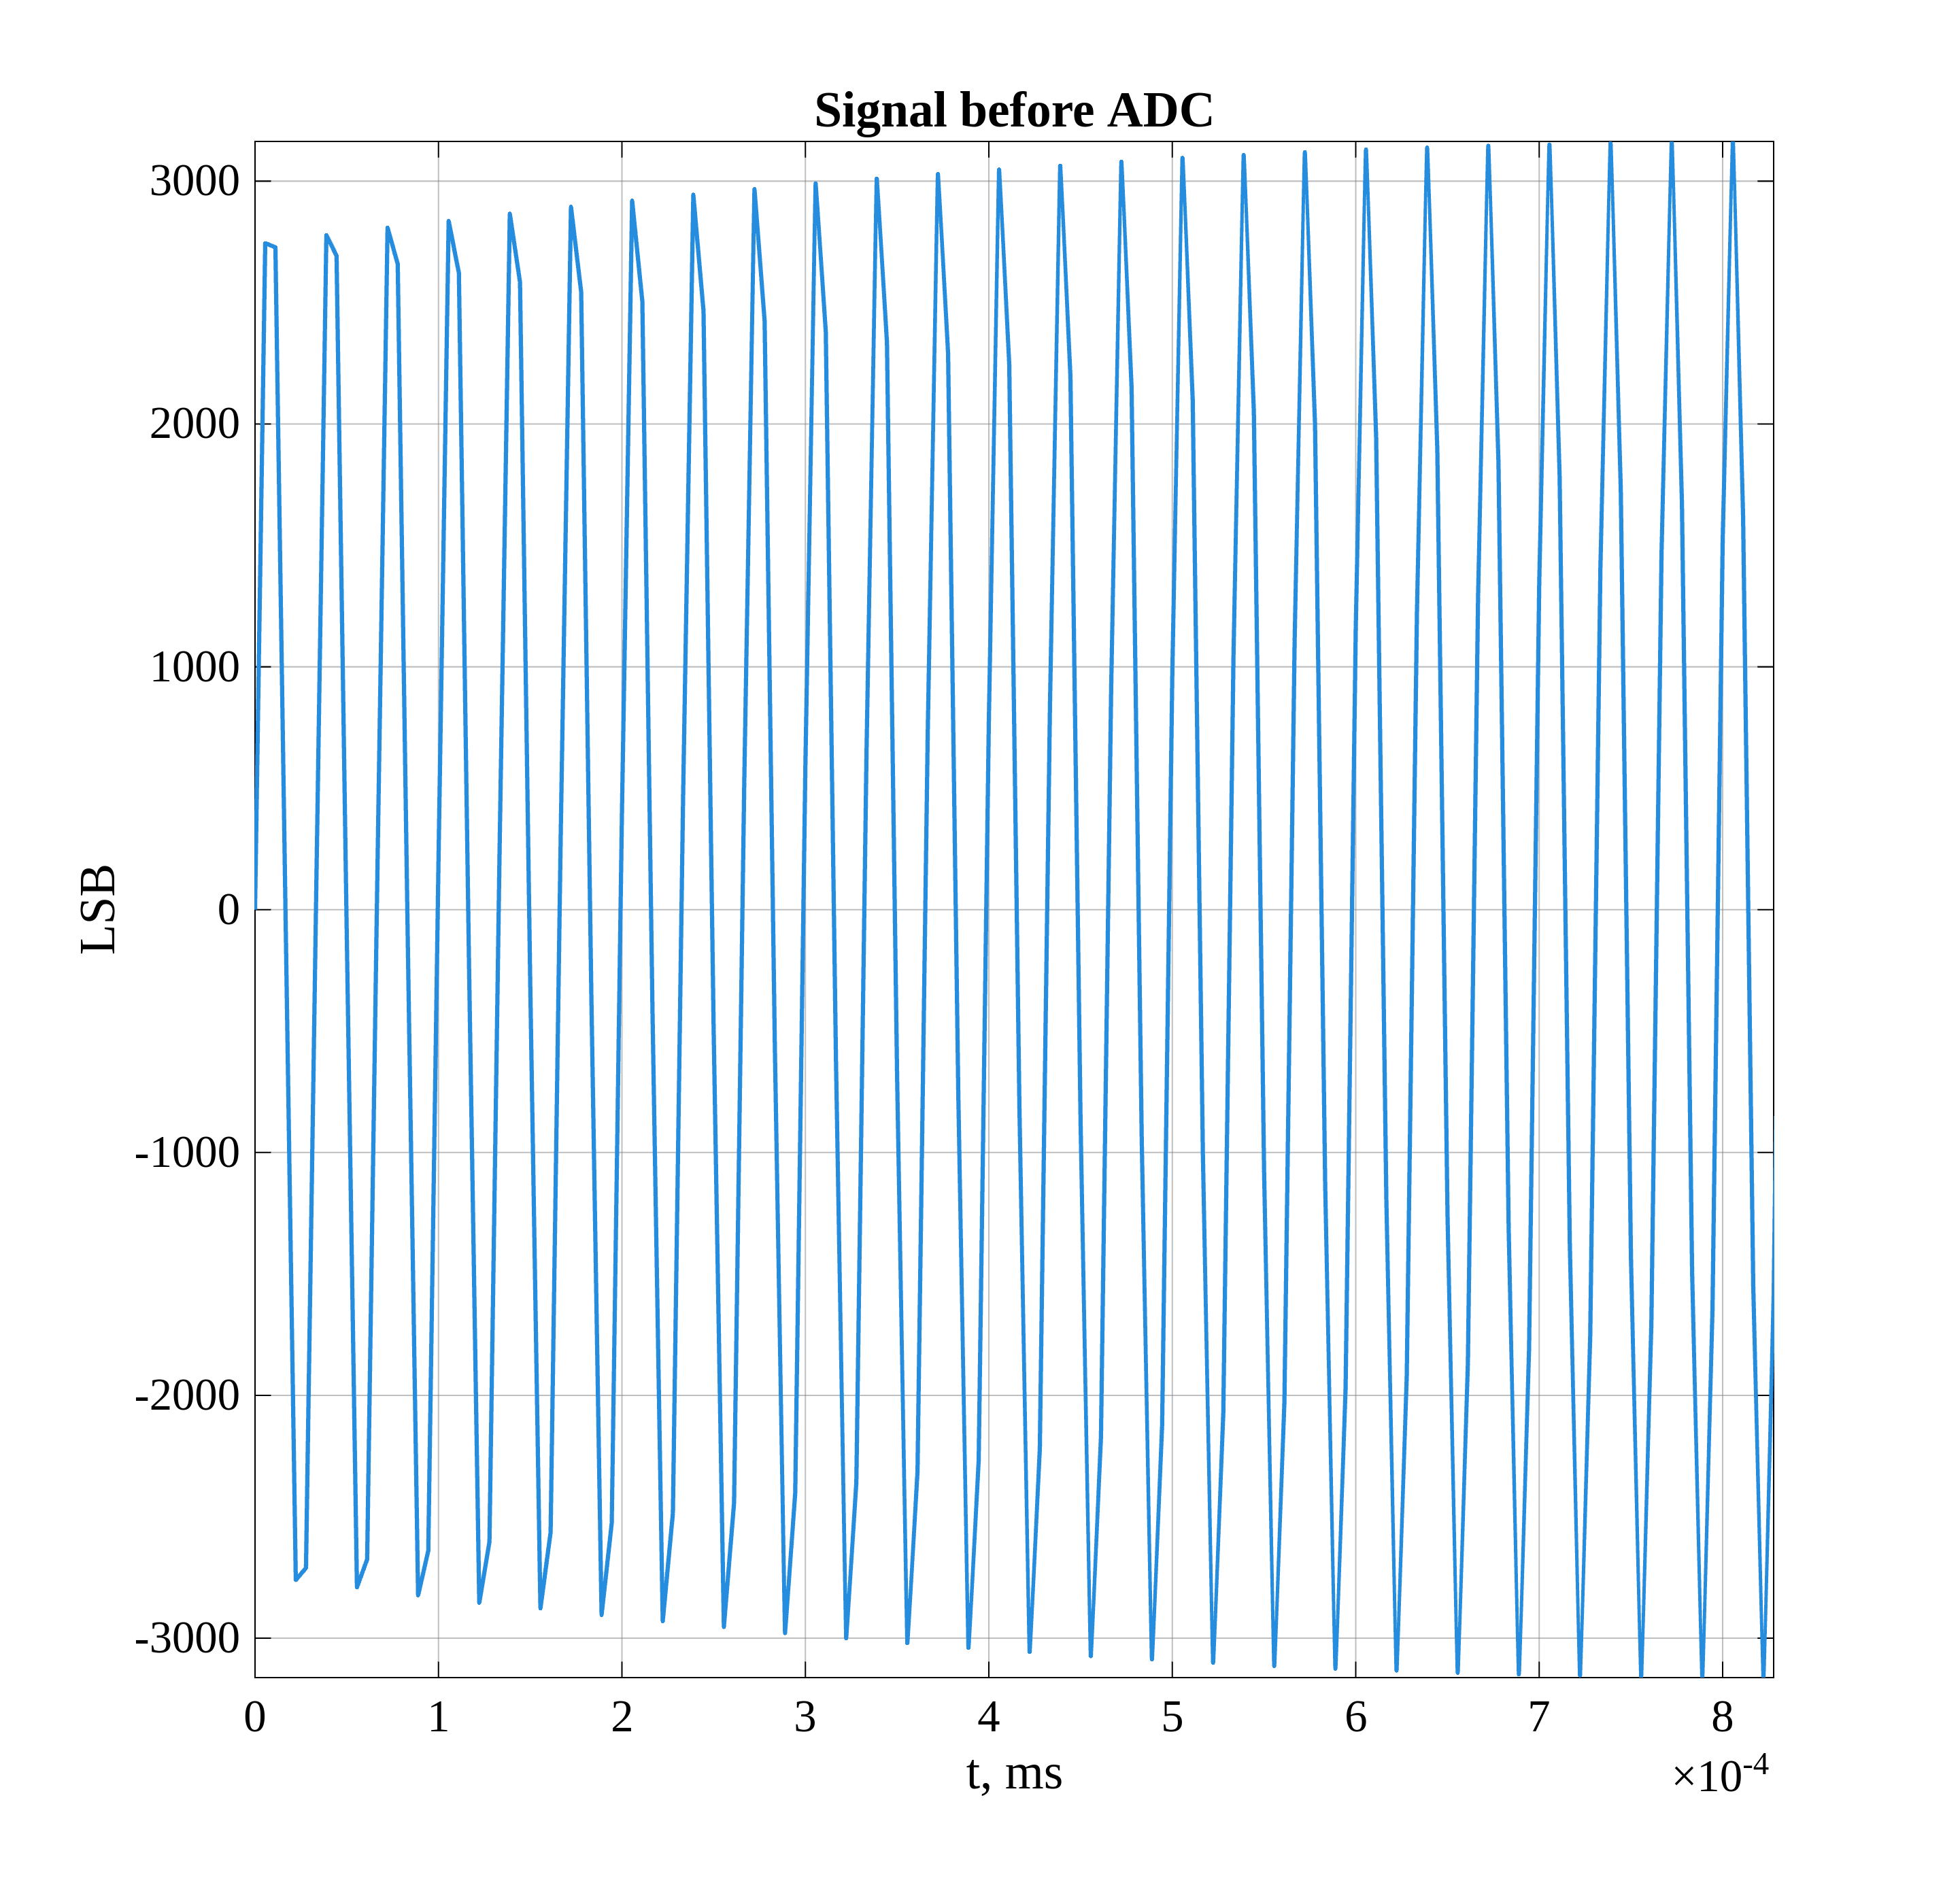
\includegraphics[width=\textwidth]{export_figs/p2_fig_01.png}
        \caption*{а) Осциллограмма}
    \end{minipage}\hfill
    \begin{minipage}{0.48\textwidth}
        \centering
        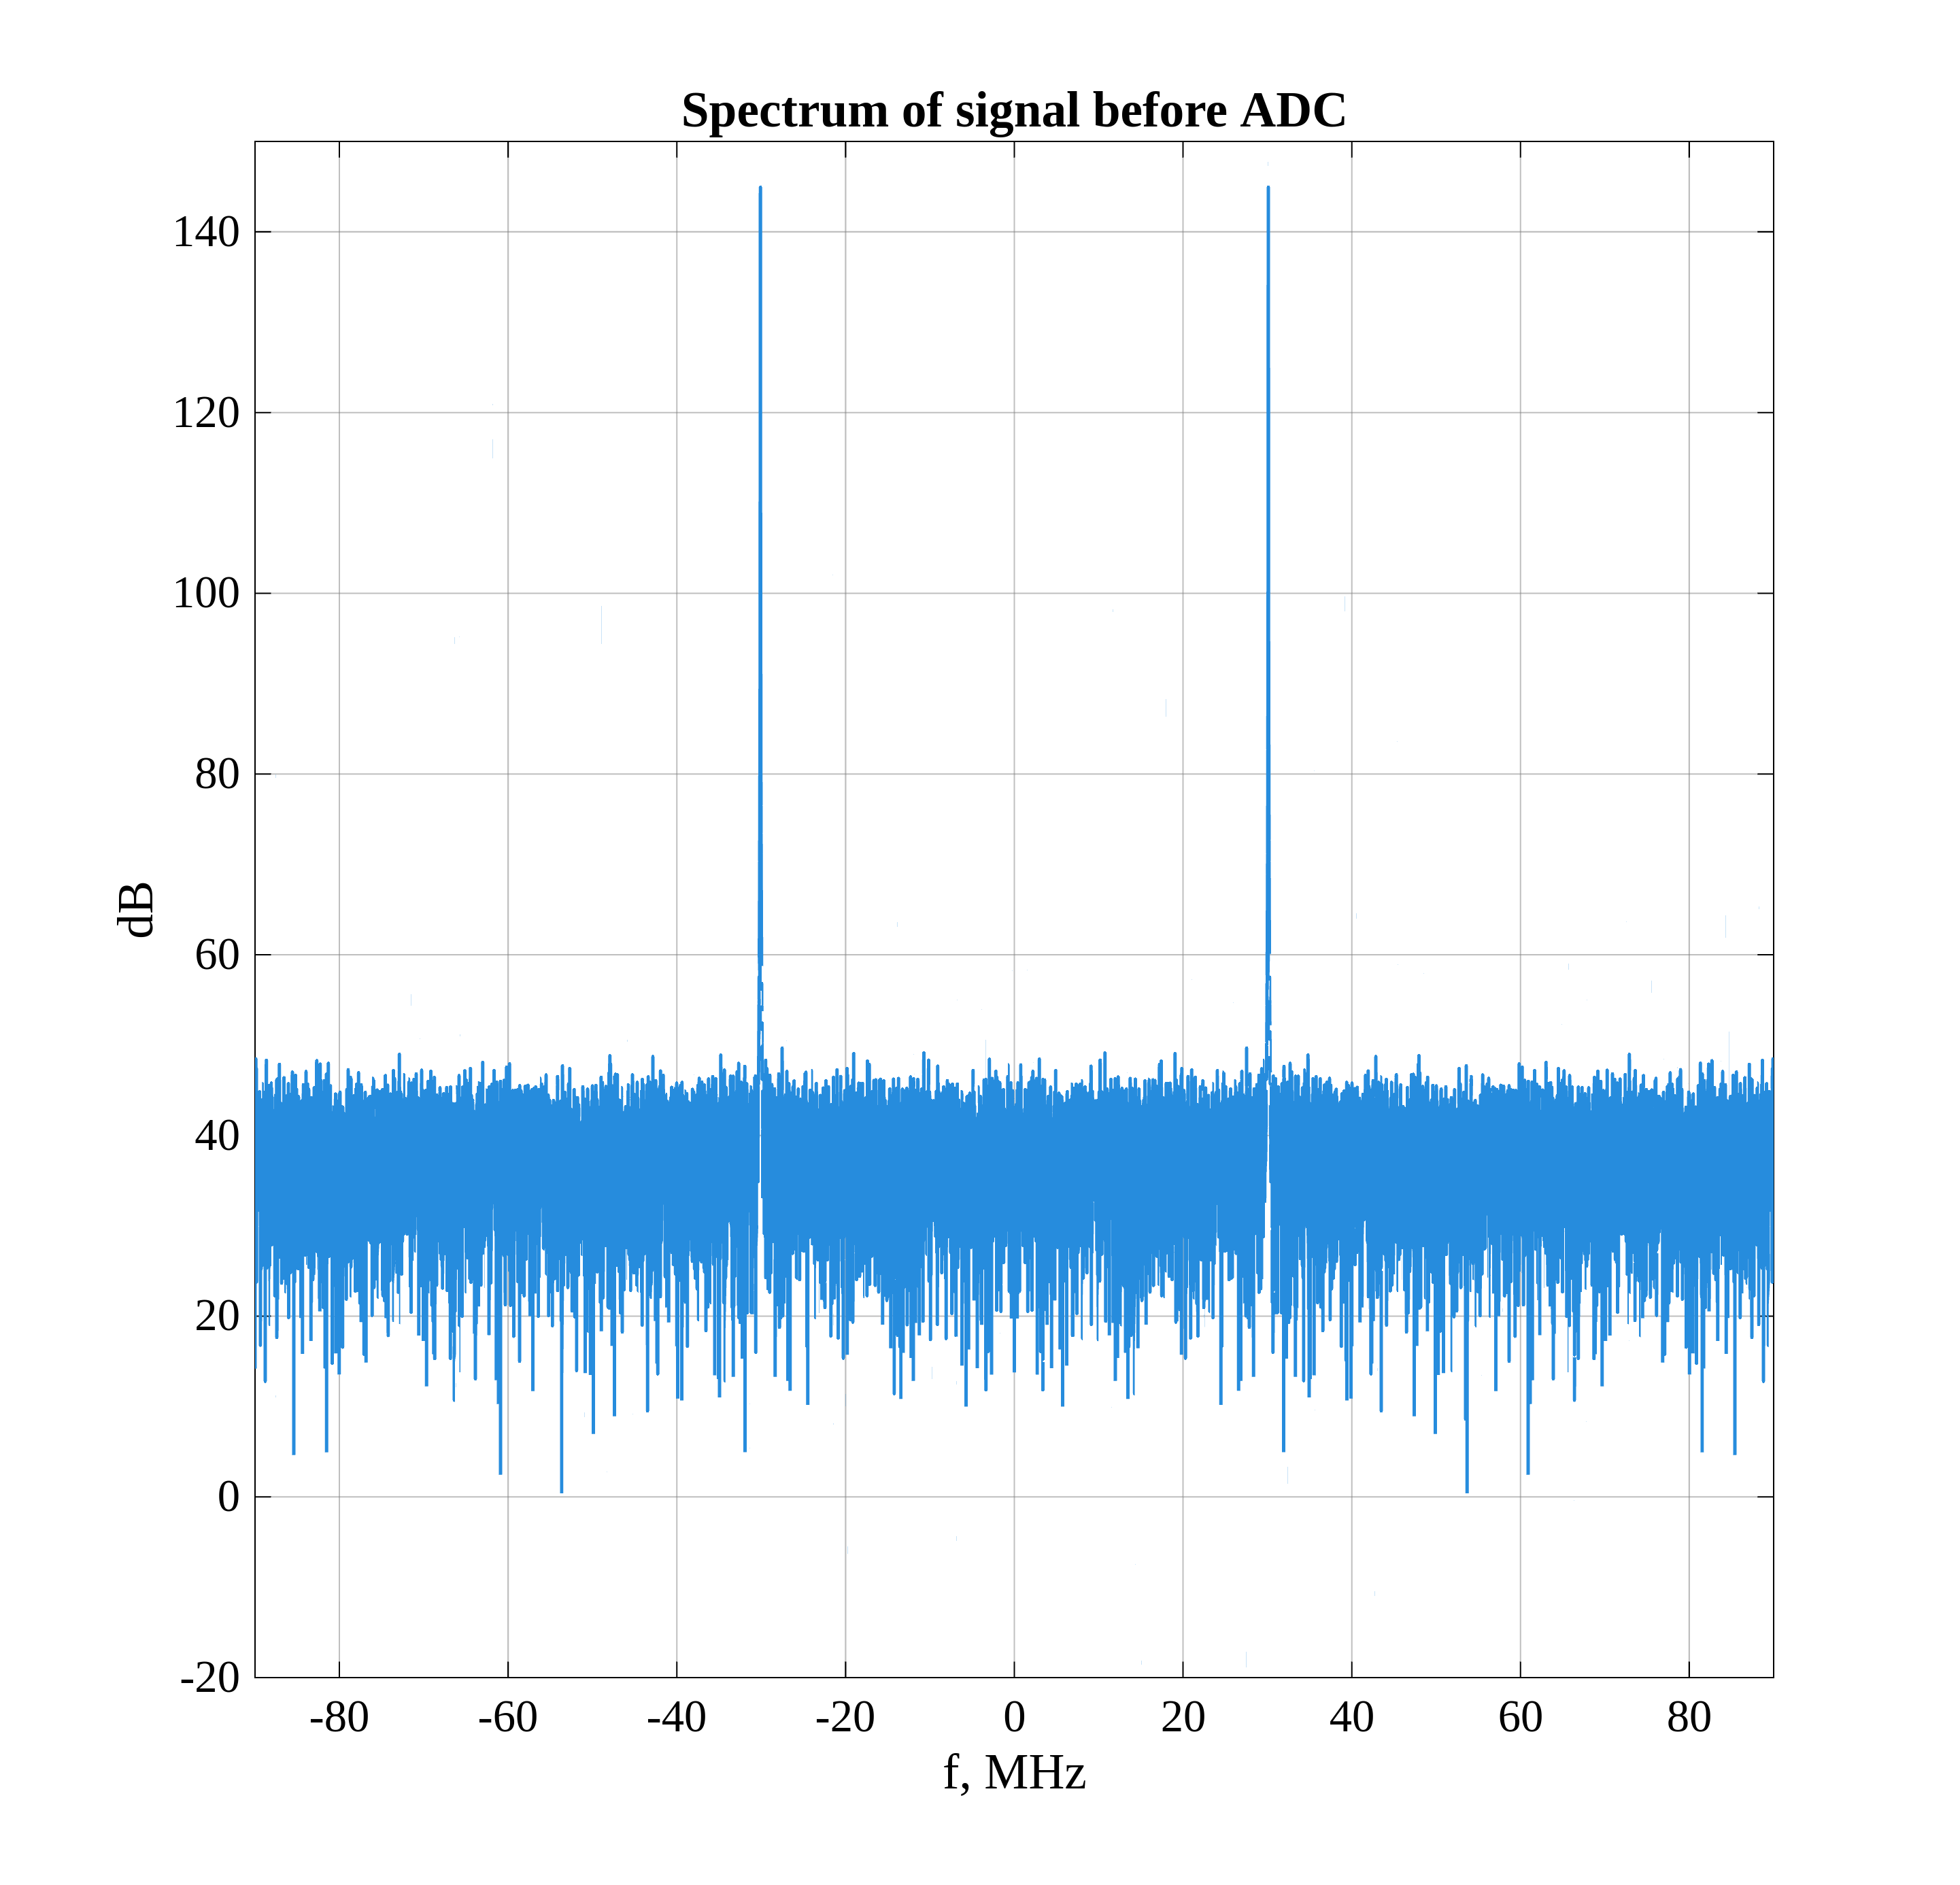
\includegraphics[width=\textwidth]{export_figs/p2_fig_02.png}
        \caption*{б) Спектр}
    \end{minipage}
    \caption{Входной сигнал до аналого-цифрового преобразования}
    \label{fig:sig_in}
\end{figure}

Далее сигнал поступает на вход 13-битного АЦП. Результат квантования по уровню и дискретизации во времени с частотой $f_s = 180$ МГц показан на рисунке \ref{fig:adc_out}. Операция квантования добавляет в сигнал специфический шум, что приводит к появлению шумового пола, ограничивающего динамический диапазон.

\begin{figure}[H]
    \centering
    \begin{minipage}{0.48\textwidth}
        \centering
        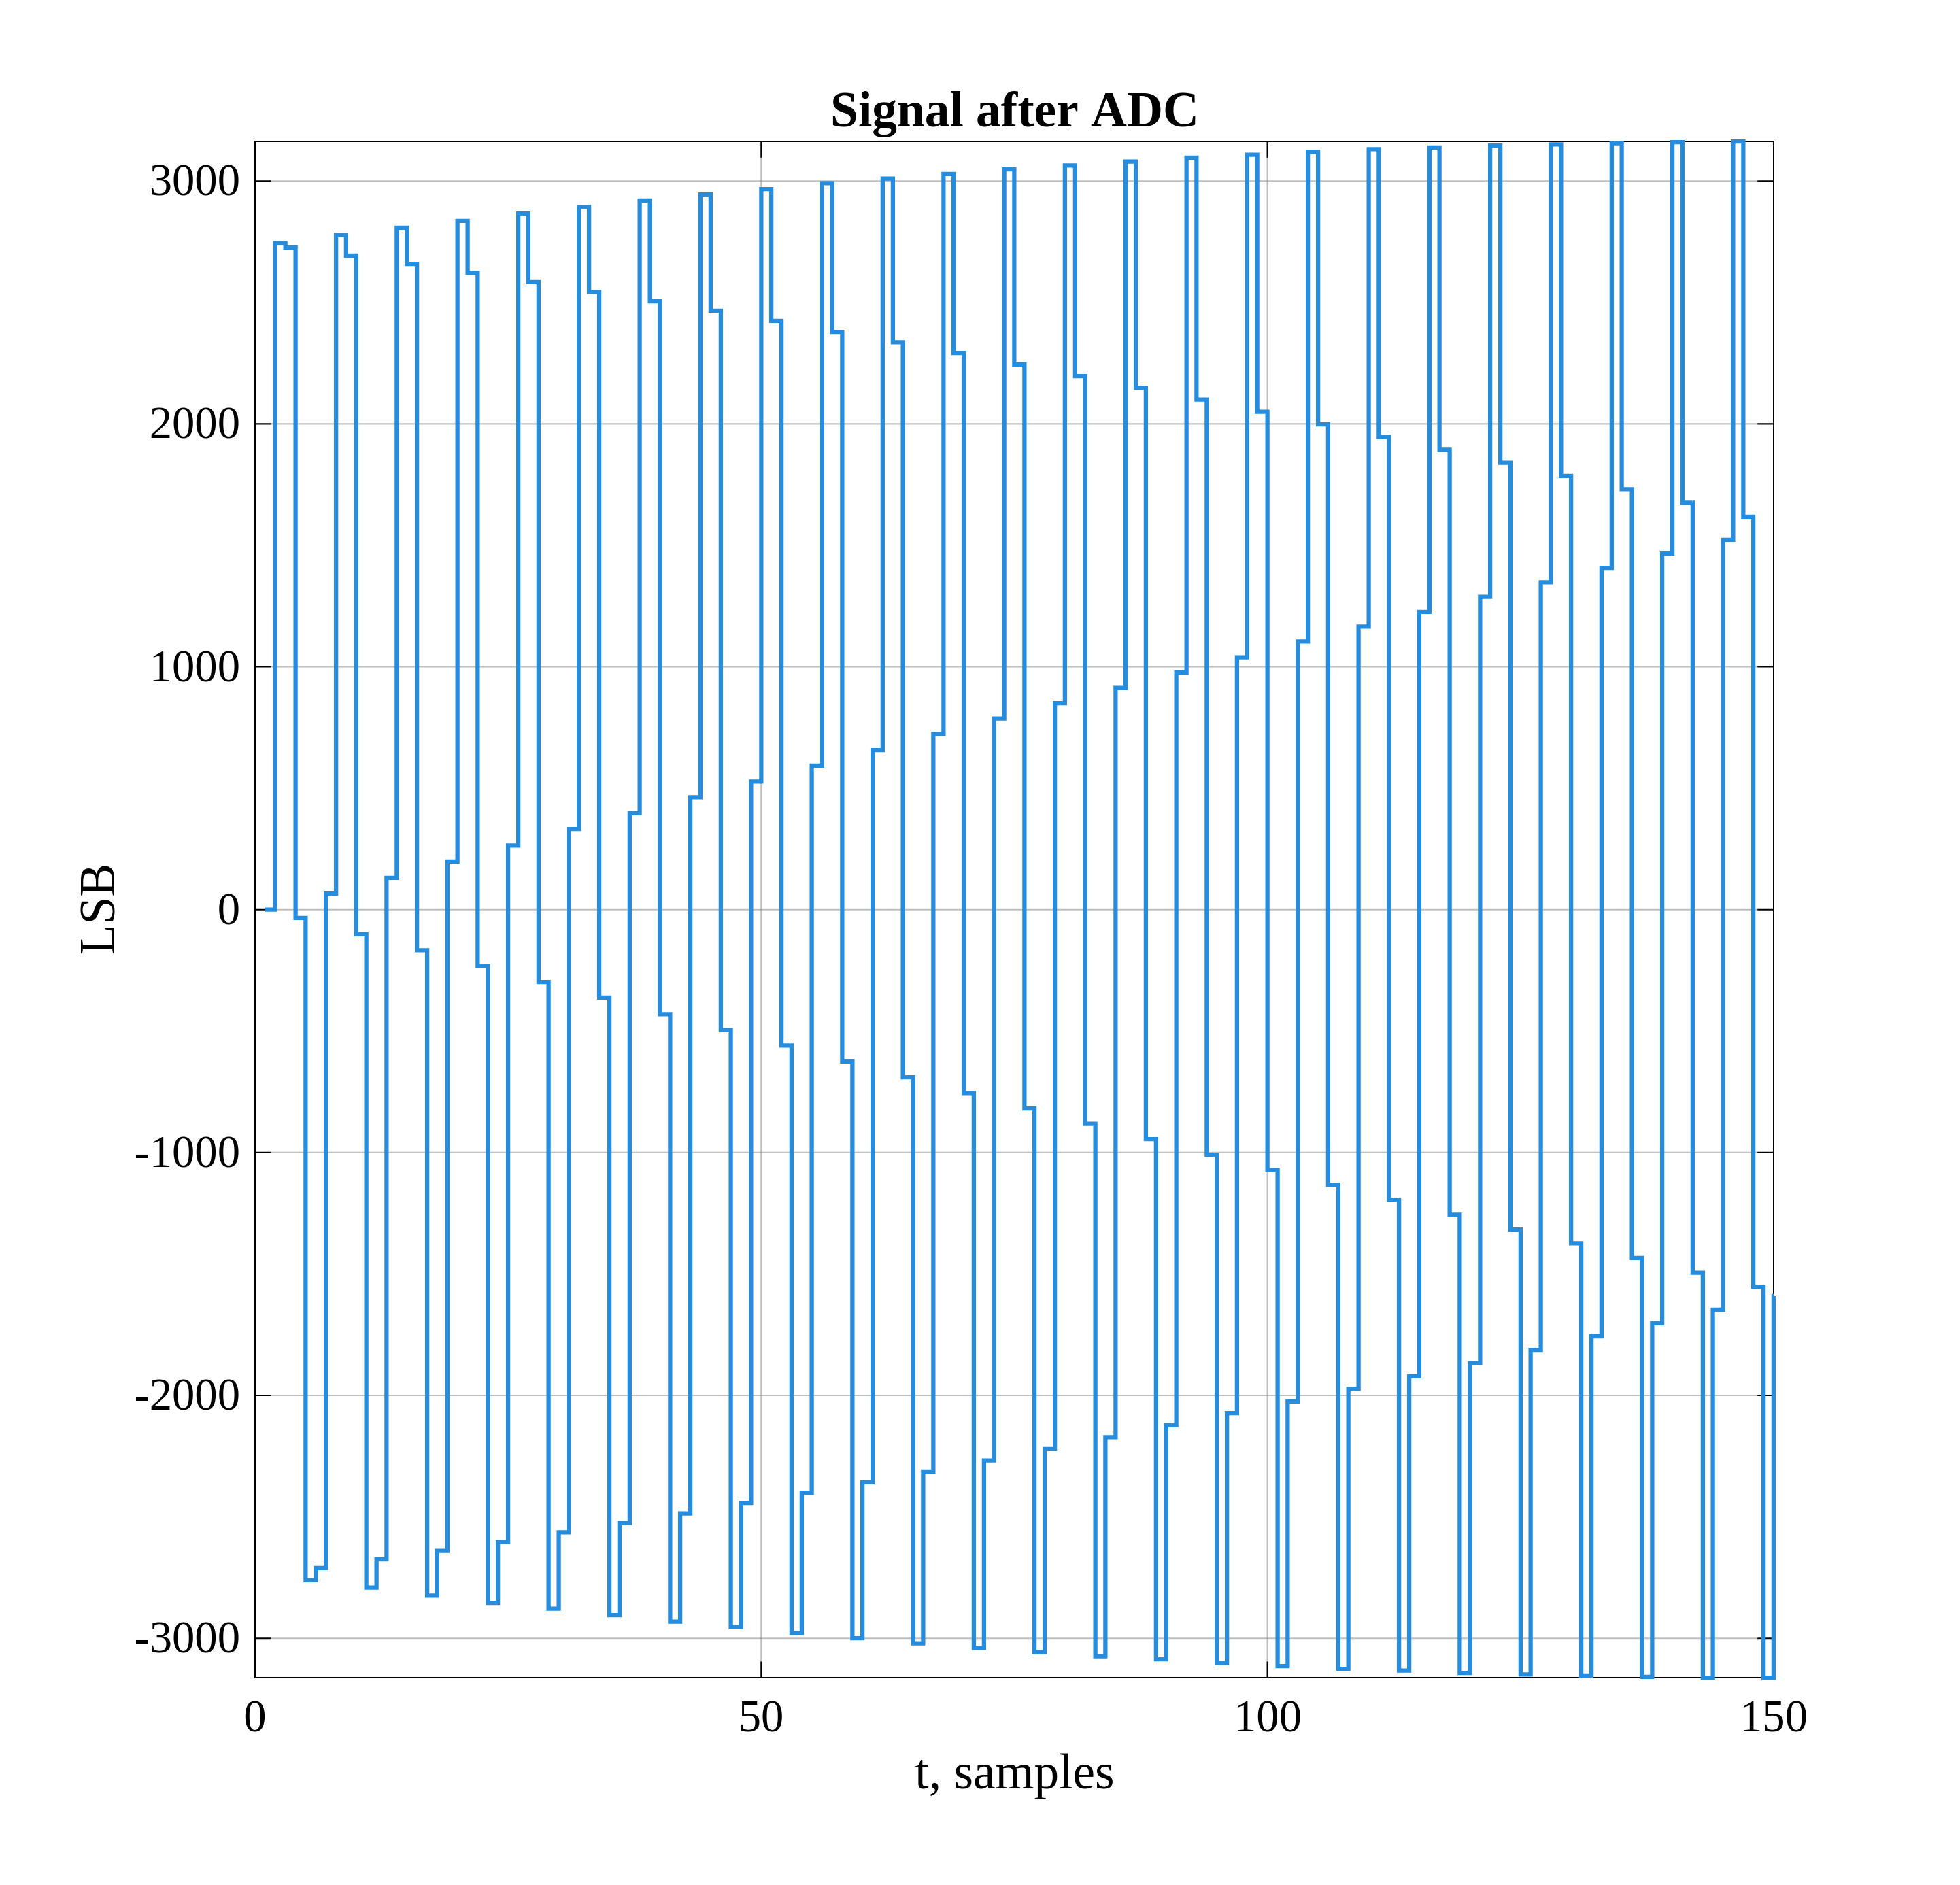
\includegraphics[width=\textwidth]{export_figs/p2_fig_03.png}
        \caption*{а) Осциллограмма}
    \end{minipage}\hfill
    \begin{minipage}{0.48\textwidth}
        \centering
        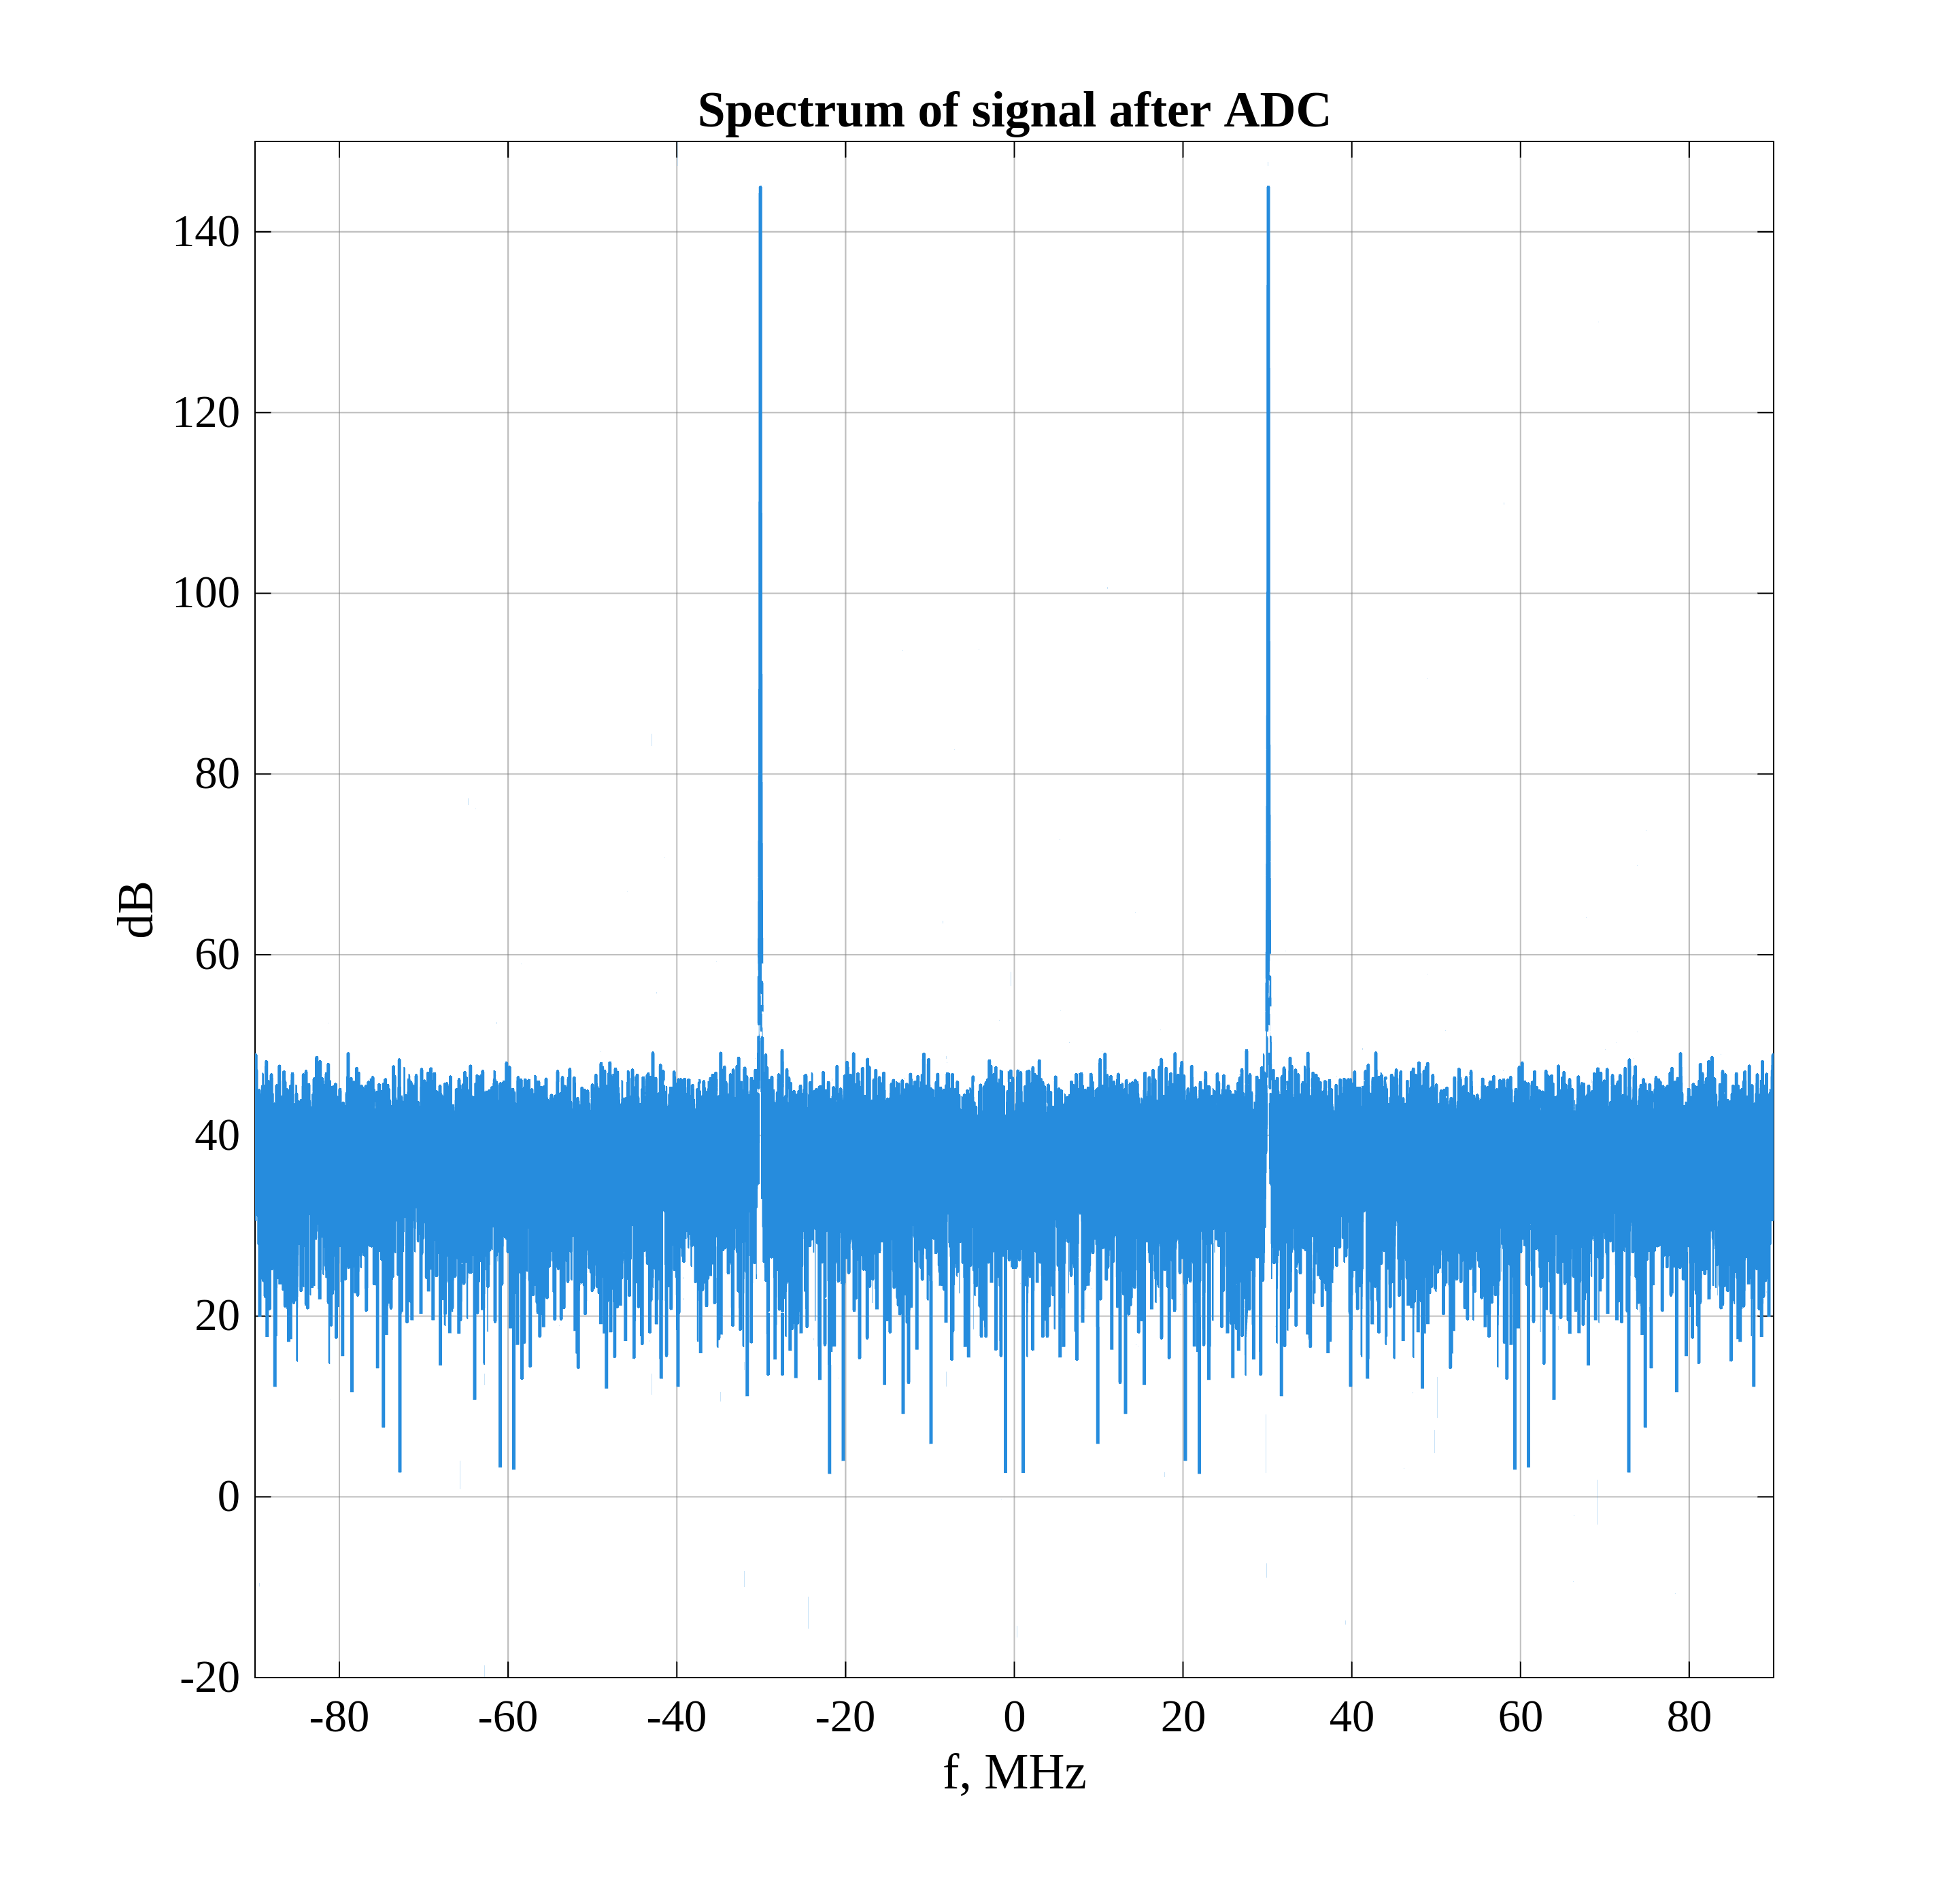
\includegraphics[width=\textwidth]{export_figs/p2_fig_04.png}
        \caption*{б) Спектр}
    \end{minipage}
    \caption{Сигнал на выходе 13-битного АЦП}
    \label{fig:adc_out}
\end{figure}

\subsection{Квадратурная демодуляция}

Для переноса спектра входного сигнала в область нулевых частот используется цифровой гетеродин (ЦГ / NCO), формирующий комплексный аналитический опорный сигнал вида:
\begin{equation}
    g[n] = g_{re}[n] - j \, g_{im}[n] = \cos(2\pi f_G n T_s) - j \sin(2\pi f_G n T_s) = e^{-j 2\pi f_G n T_s}.
    \label{eq:nco_exp}
\end{equation}

\begin{figure}[H]
    \centering
    \begin{minipage}{0.48\textwidth}
        \centering
        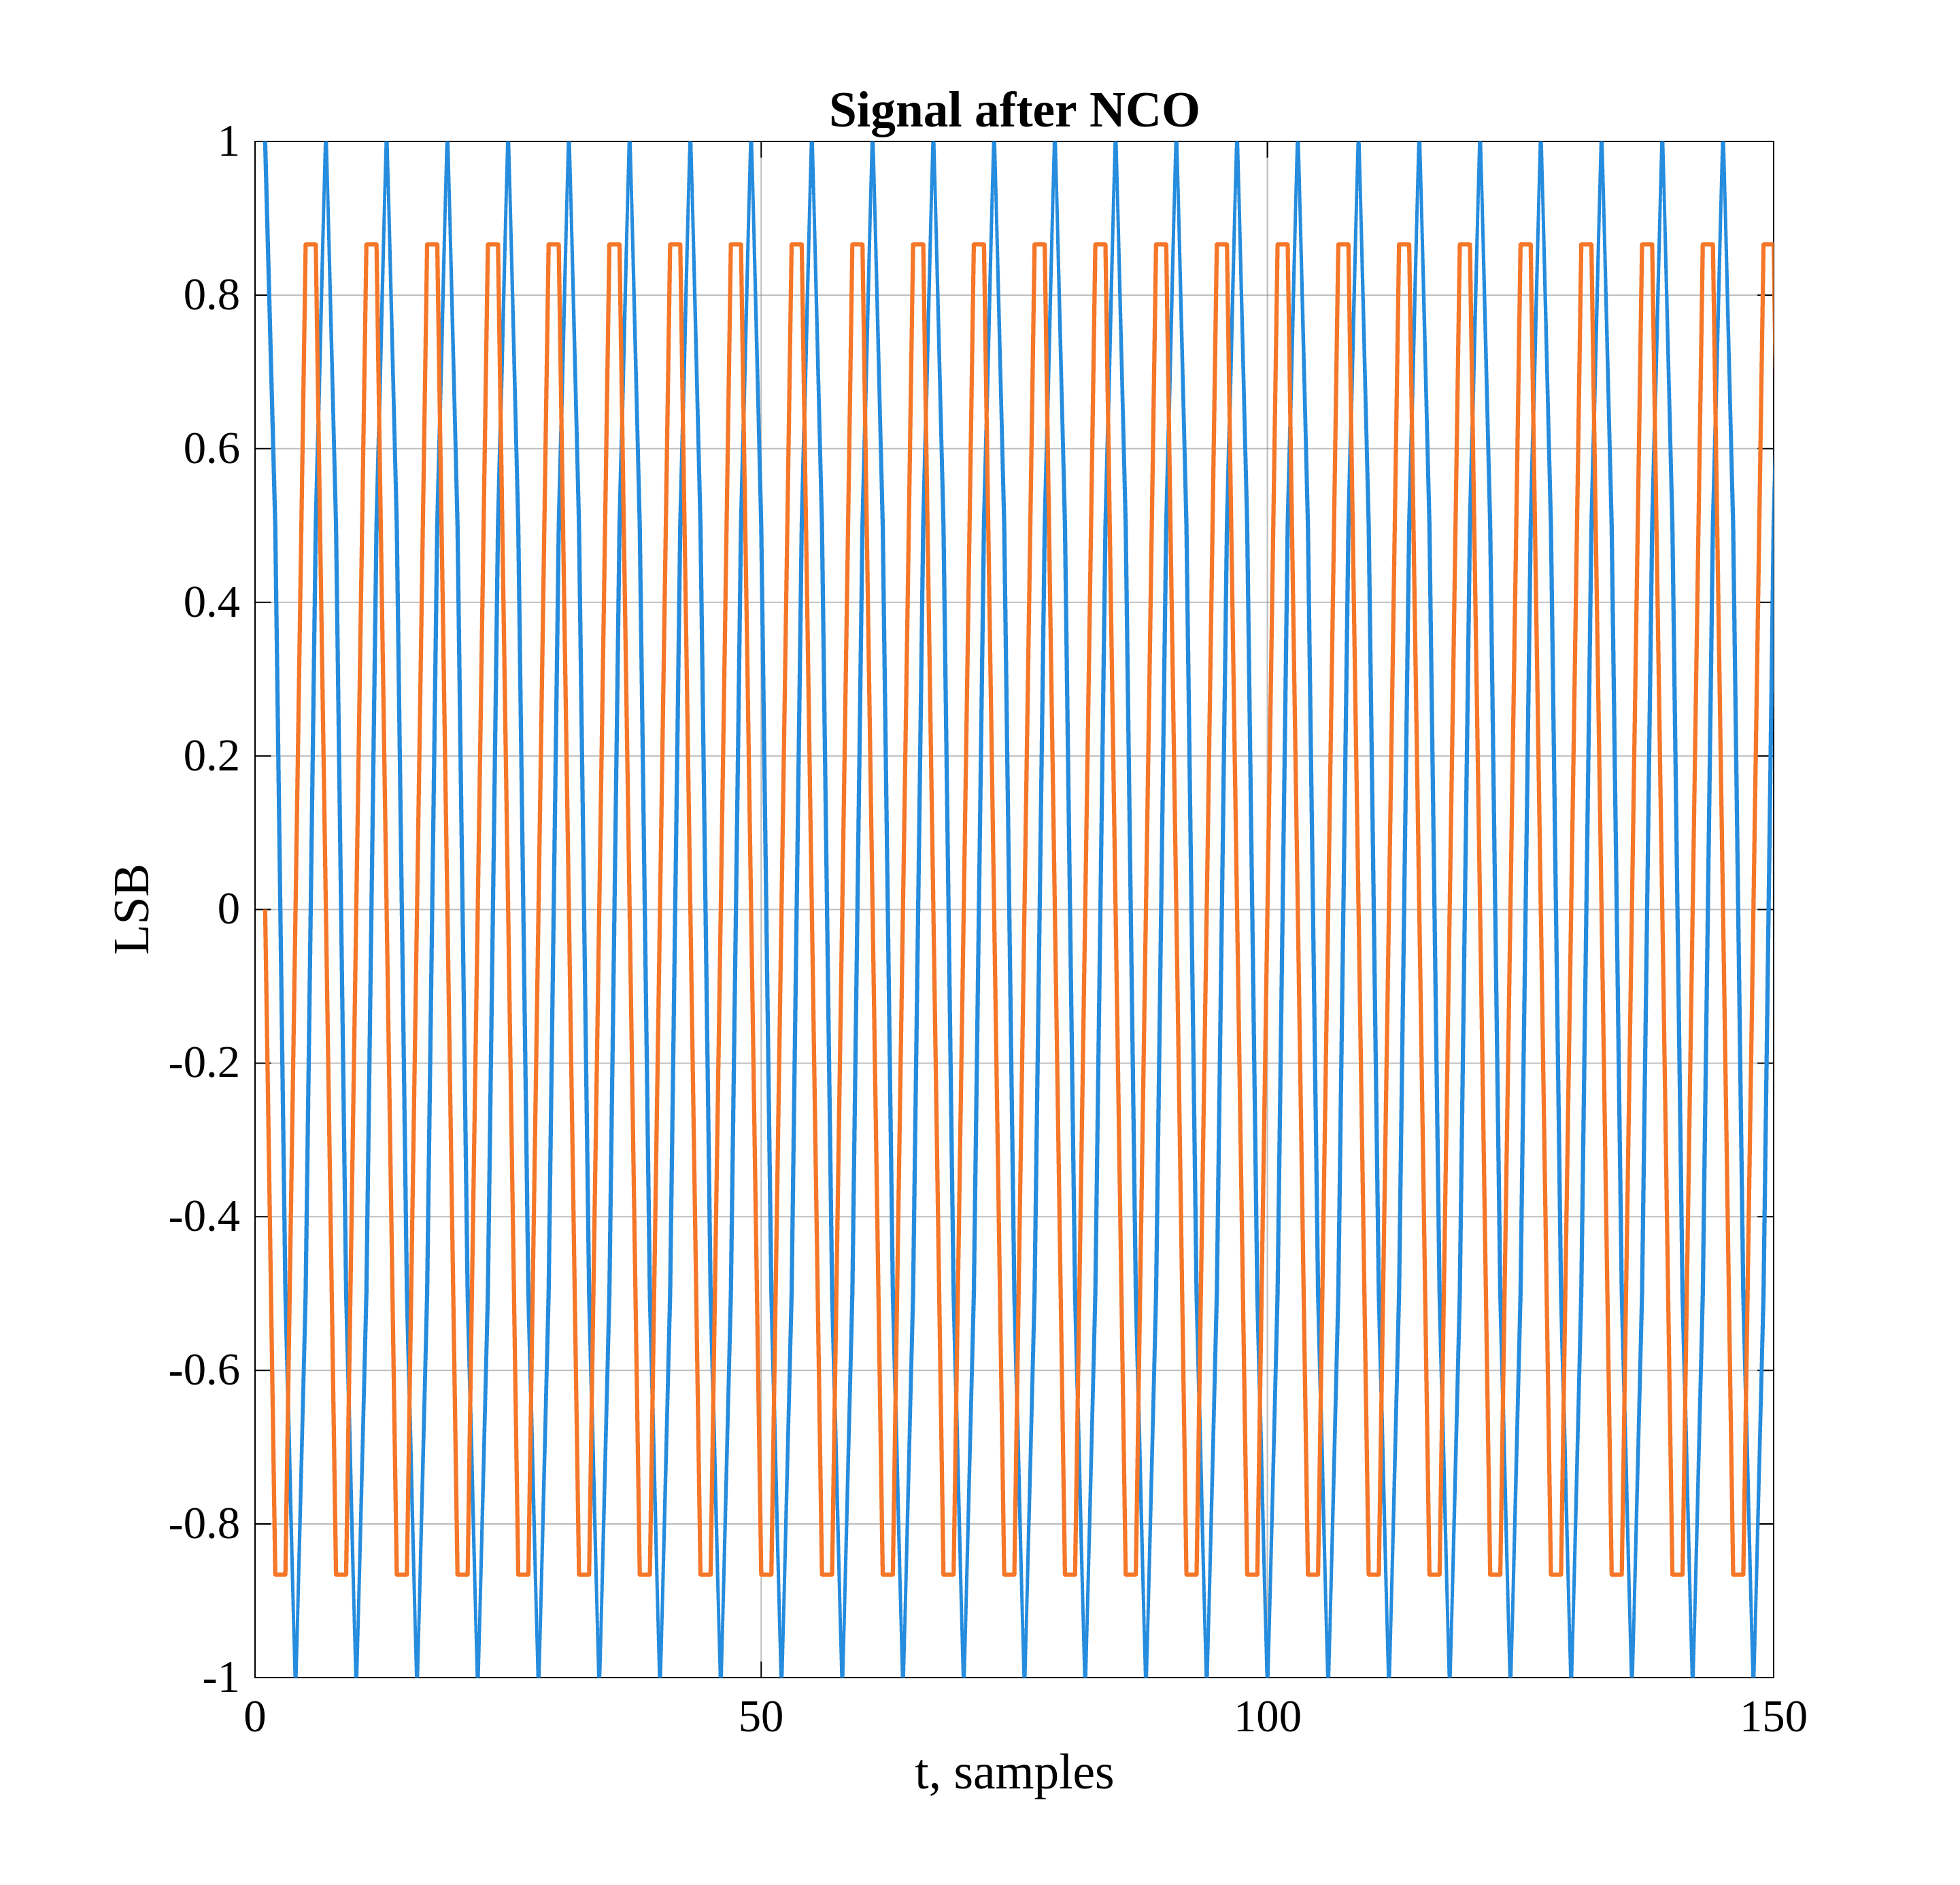
\includegraphics[width=\textwidth]{export_figs/p2_fig_05.png}
        \caption*{а) Квадратуры ЦГ}
    \end{minipage}\hfill
    \begin{minipage}{0.48\textwidth}
        \centering
        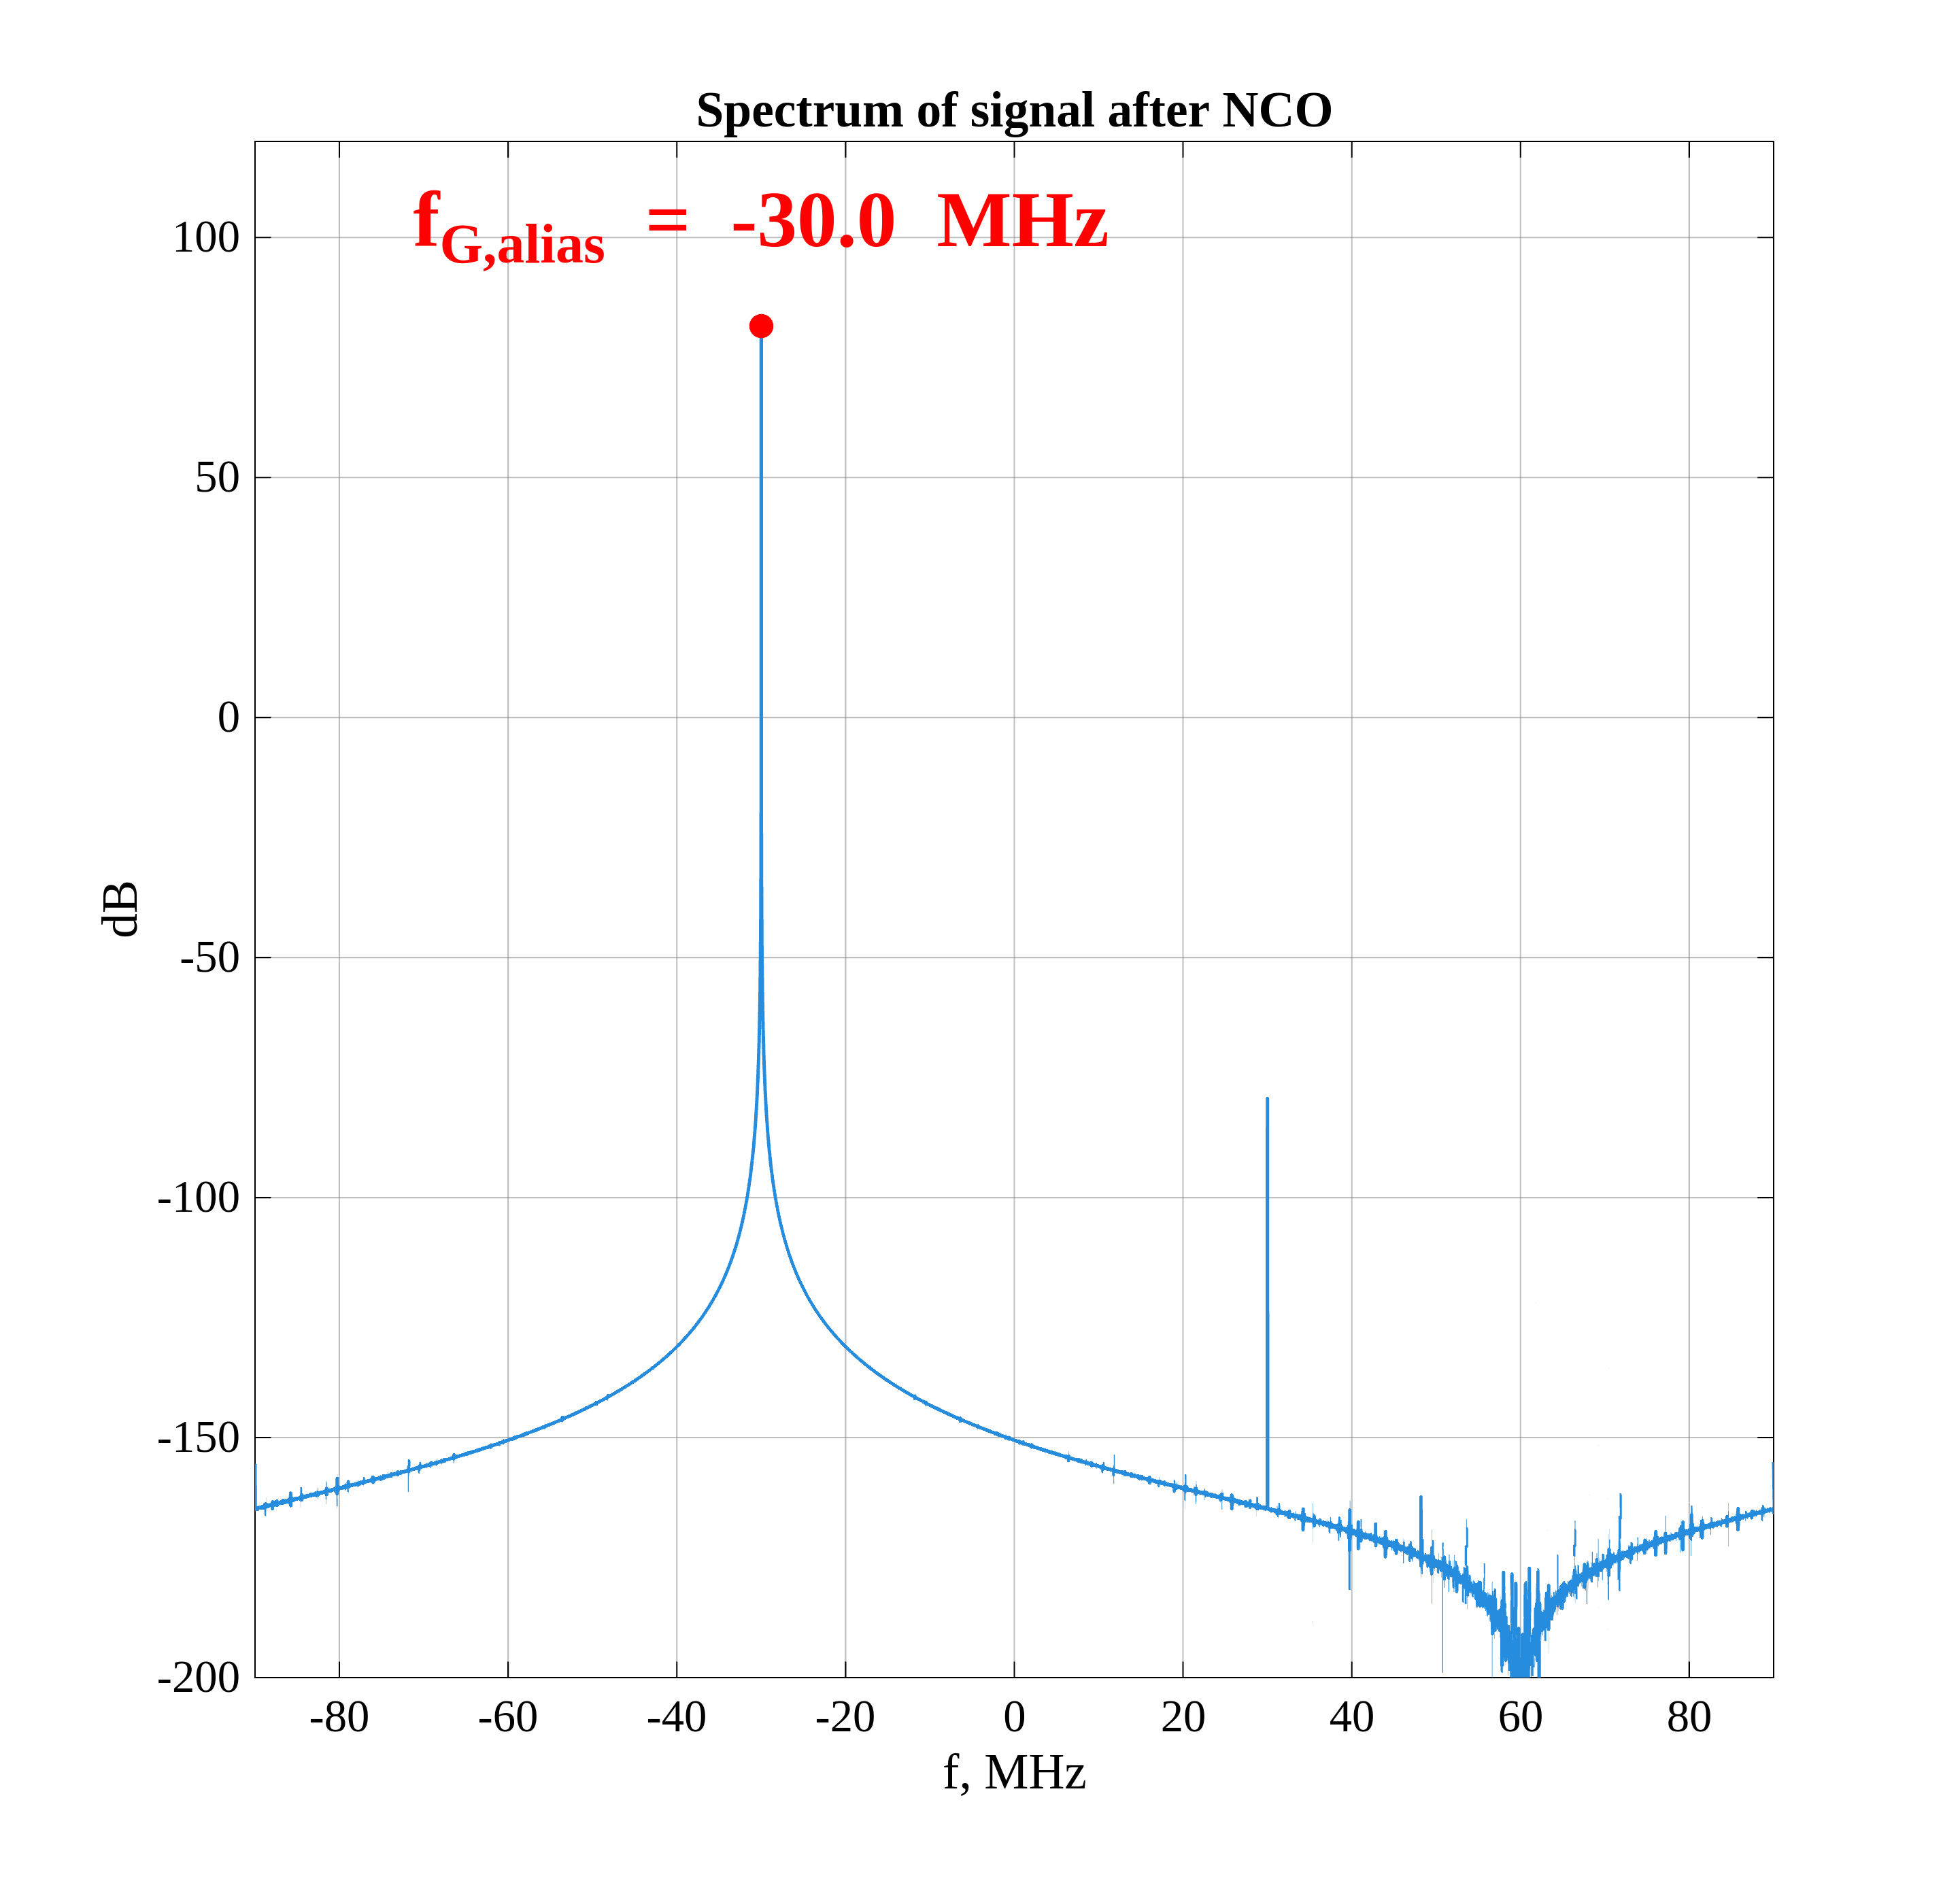
\includegraphics[width=\textwidth]{export_figs/p2_fig_06.png}
        \caption*{б) Спектр ЦГ}
    \end{minipage}
    \caption{Комплексный опорный сигнал цифрового гетеродина (NCO)}
    \label{fig:nco_sig}
\end{figure}

На рисунке \ref{fig:nco_sig} представлены временные реализации квадратур и спектр опорного сигнала. Спектр комплексной экспоненты $e^{-j 2\pi f_G t}$ содержит единственную гармонику на отрицательной частоте. С учетом дискретизации с частотой $f_s = 180$ МГц частота гетеродина $f_G = 210.0$ МГц претерпевает стробоскопический перенос (алиасинг) во вторую зону Найквиста:
\begin{equation}
    f_{G,\text{alias}} = - (f_G - f_s) = -(210.0 - 180.0) = -30.0\text{ МГц}.
\end{equation}

Подавление положительной спектральной составляющей на $+30$ МГц достигается за счет вычитания квадратур ($I - jQ$), что предотвращает наложение зеркального канала при понижающем преобразовании частоты.

\begin{figure}[H]
    \centering
    \begin{minipage}{0.48\textwidth}
        \centering
        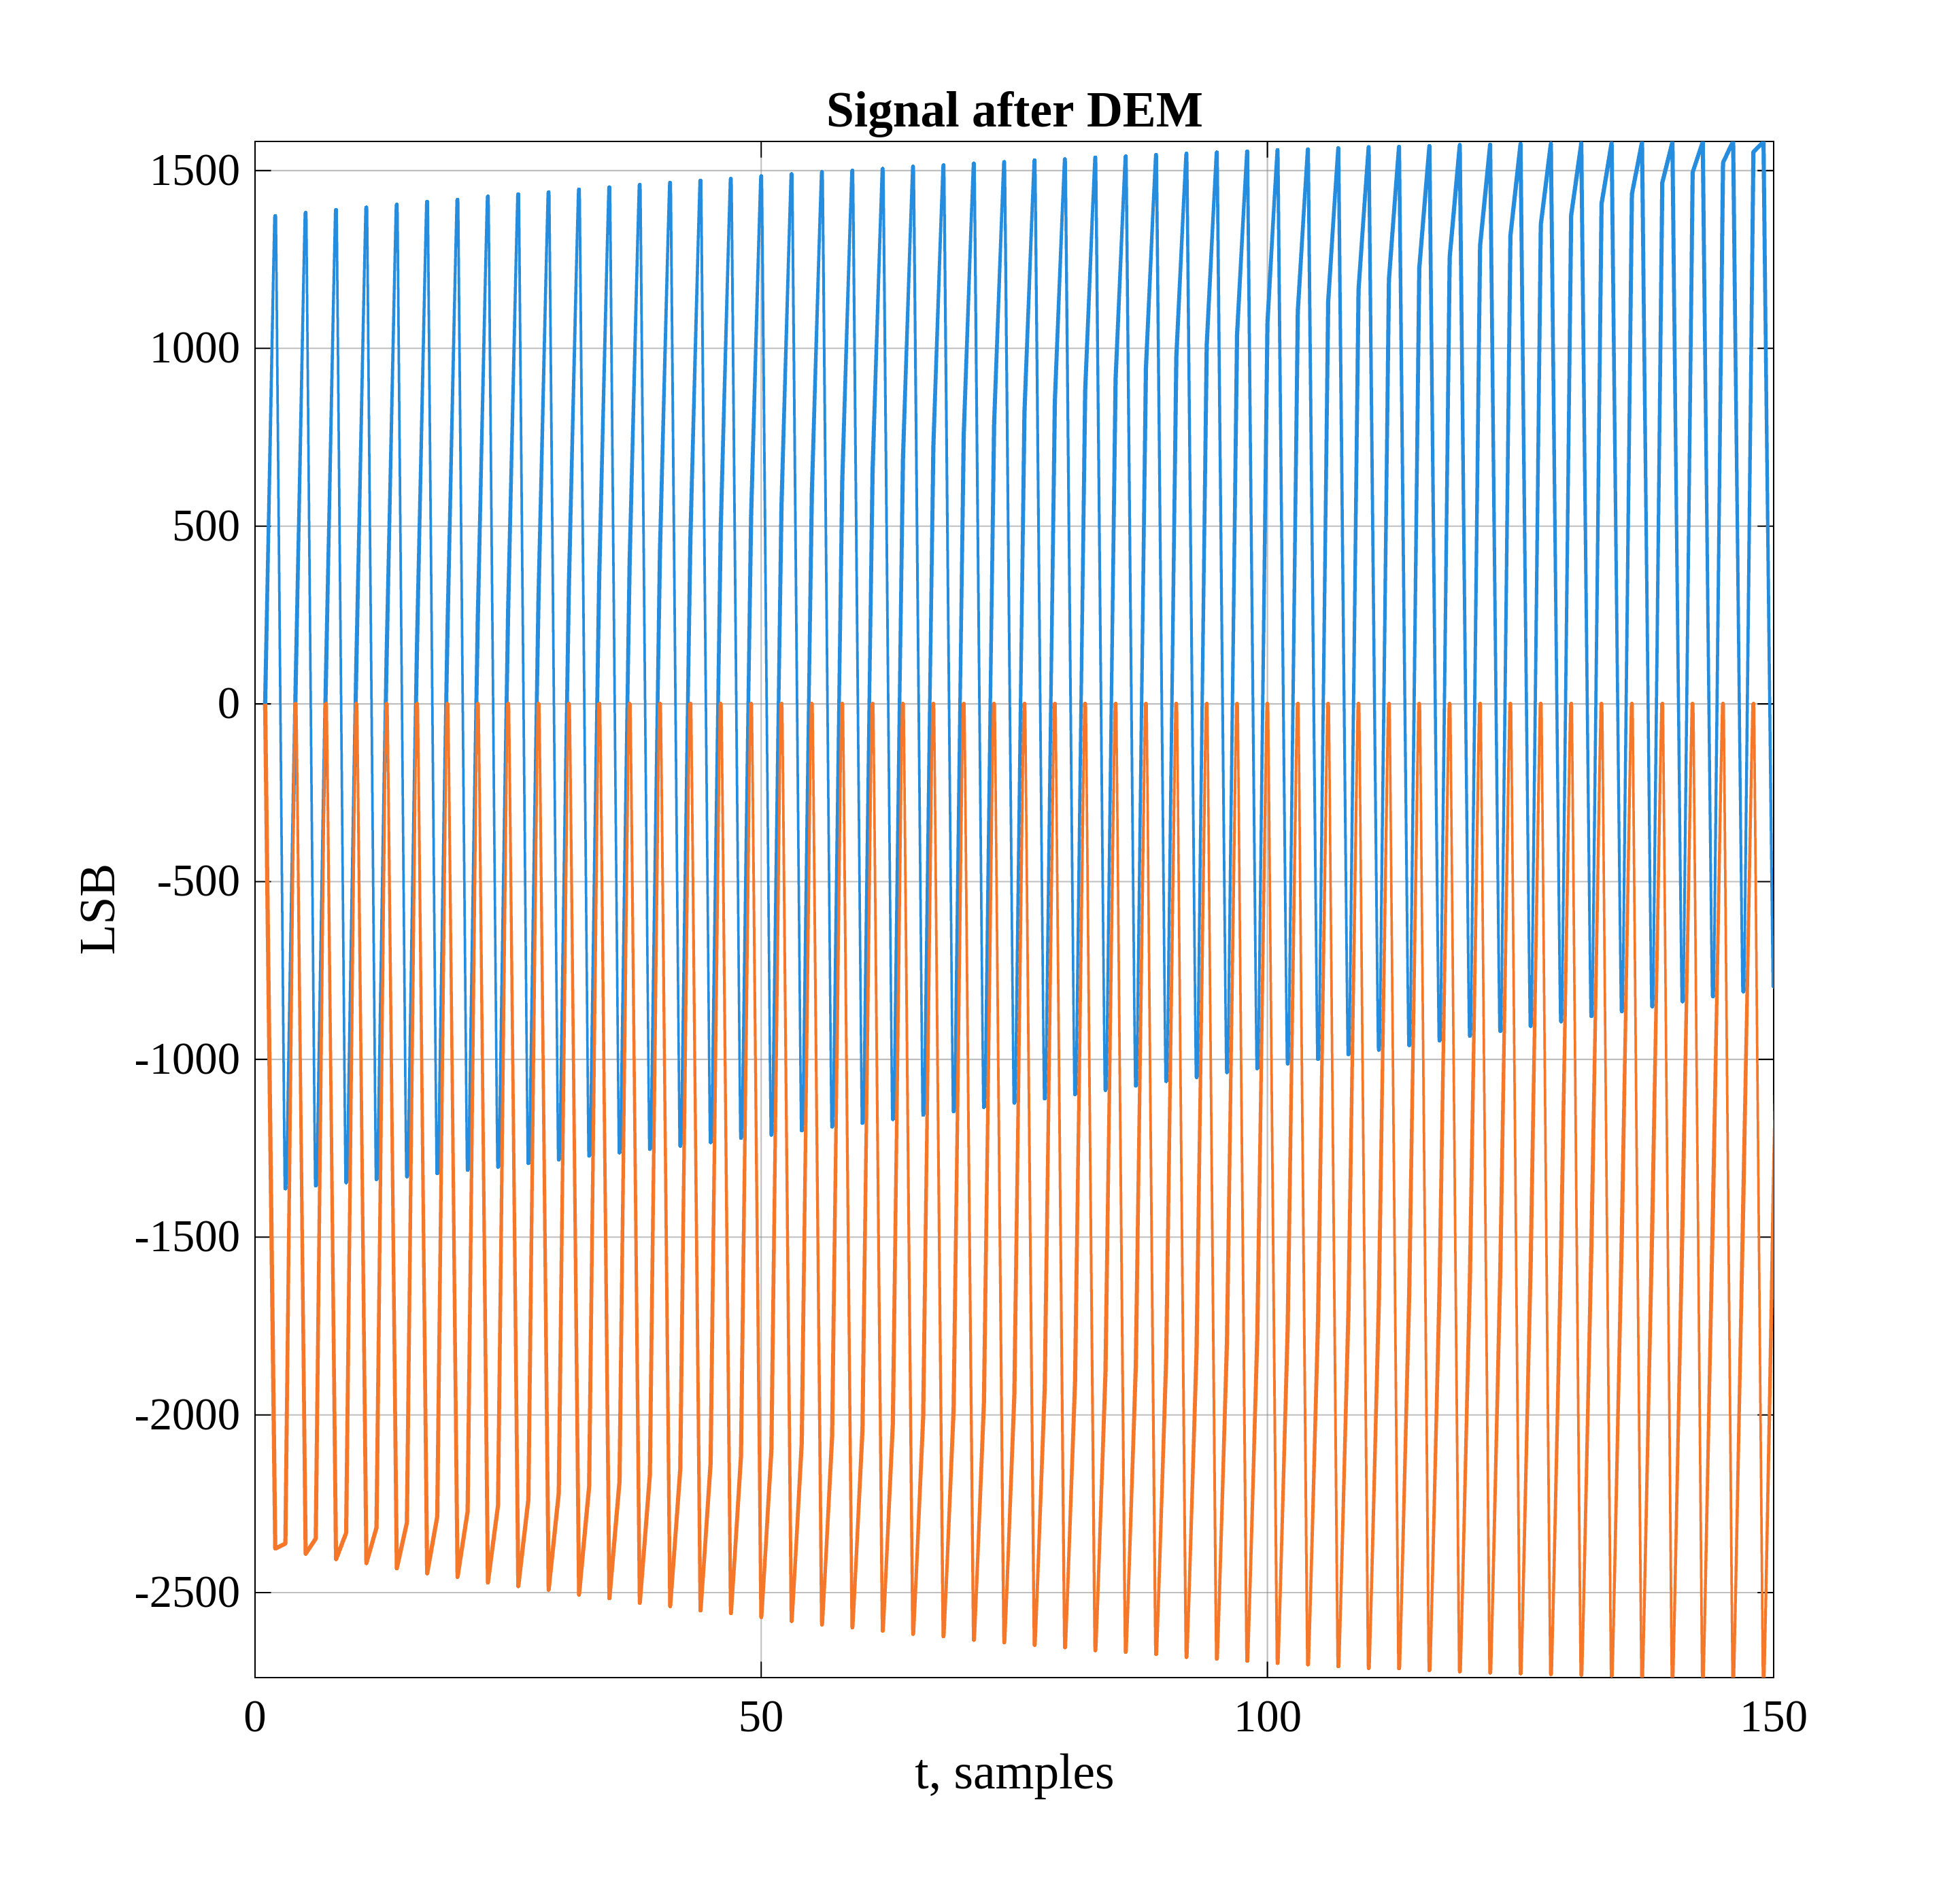
\includegraphics[width=\textwidth]{export_figs/p2_fig_07.png}
        \caption*{а) Осциллограмма}
    \end{minipage}\hfill
    \begin{minipage}{0.48\textwidth}
        \centering
        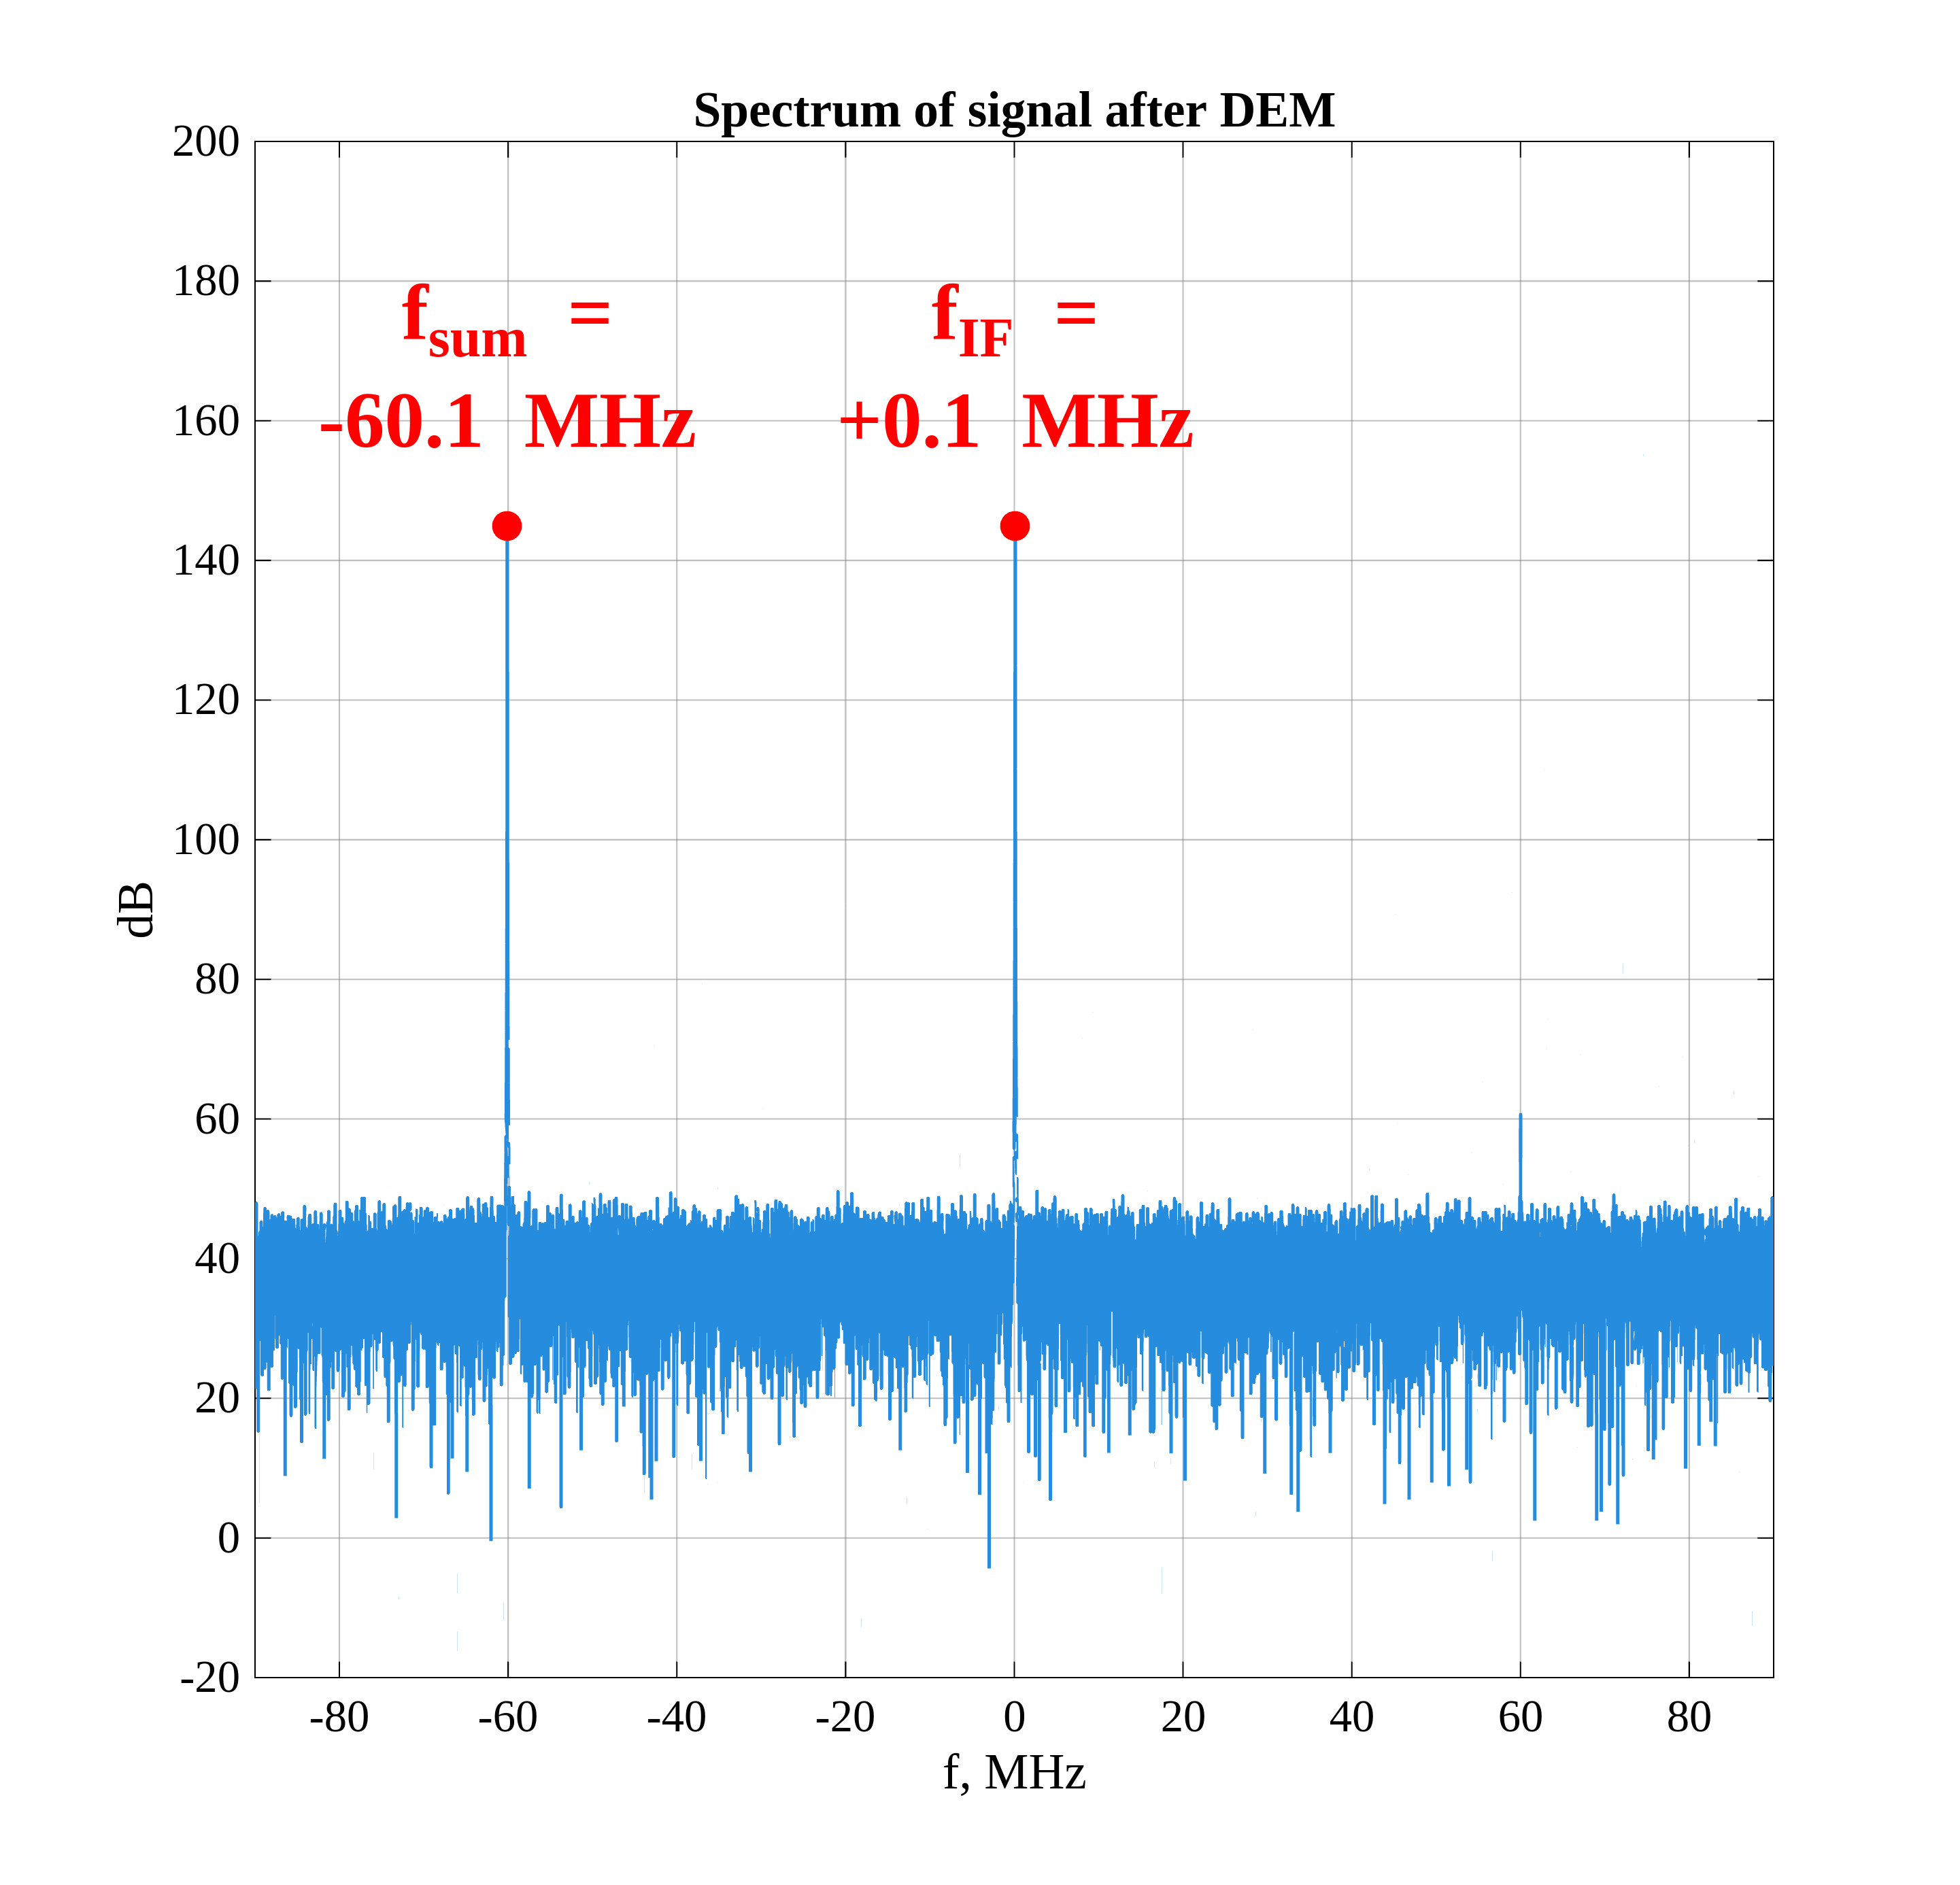
\includegraphics[width=\textwidth]{export_figs/p2_fig_08.png}
        \caption*{б) Спектр}
    \end{minipage}
    \caption{Сигнал после цифрового квадратурного смесителя (демодулятора)}
    \label{fig:dem_out}
\end{figure}

Как видно из приведенного на рисунке \ref{fig:dem_out}б спектра, на выходе смесителя формируются две выраженные спектральные компоненты:
\begin{enumerate}
    \item \textbf{Полезная разностная составляющая} на низкой промежуточной частоте:
    \begin{equation}
        f_{IF} = f_{c,\text{alias}} - f_{G,\text{alias}} = 30.1 - 30.0 = +0.1\text{ МГц};
    \end{equation}
    \item \textbf{Паразитная суммарная составляющая} на удвоенной частоте со знаком «минус» (обусловленным знаком комплексной экспоненты гетеродина):
    \begin{equation}
        f_{sum} = -(f_{c,\text{alias}} + f_{G,\text{alias}}) = -(30.1 + 30.0) = -60.1\text{ МГц}.
    \end{equation}
\end{enumerate}
Подавление высокочастотной составляющей на $-60.1$ МГц и выделение полезной компоненты на $+0.1$ МГц возлагается на последующий каскад децимирующих фильтров.

\subsection{Многоступенчатая фильтрация и децимация}

Для подавления паразитной суммарной высокочастотной составляющей смесителя ($f_{sum} = -60.1$ МГц), устранения шумов квантования и понижения частоты дискретизации тракта в $R=10$ раз применяется двухкаскадная схема фильтрации.

Первым каскадом является гребенчатый фильтр-интегратор (CIC-фильтр 8-го порядка), реализующий эффективную децимацию без использования аппаратных умножителей. В результате децимации частота дискретизации снижается с $f_s = 180$ МГц до $f_{sv} = f_s / R = 18$ МГц, а новая зона Найквиста определяется диапазоном $[-f_{sv}/2;\, +f_{sv}/2] = [-9;\, +9]$ МГц. 

При этом высокочастотная составляющая $f_{sum} = -60.1$ МГц из-за эффекта наложения спектров переносится во вновь сформированную зону Найквиста:
\begin{equation}
    f_{sum,\text{new}} = f_{sum} + 3 f_{sv} = -60.1 + 3 \cdot 18.0 = -6.1\text{ МГц}.
    \label{eq:cic_alias}
\end{equation}

Благодаря тому, что передаточная характеристика CIC-фильтра имеет глубокие нули АЧХ на частотах, кратных новой частоте дискретизации, данная гармоника подавляется практически до уровня шума. 

На рисунке \ref{fig:cic_out} приведены осциллограмма и спектр комплексного сигнала после CIC-фильтра. На осциллограмме (рис. \ref{fig:cic_out}а) в окне 450 отсчетов четко различимы 2.5 периода полезного гармонического колебания частоты $f_{IF} = 0.1$ МГц (рис. \ref{fig:cic_out}б) с квадратурным сдвигом фаз $90^\circ$.

\begin{figure}[H]
    \centering
    \begin{minipage}{0.48\textwidth}
        \centering
        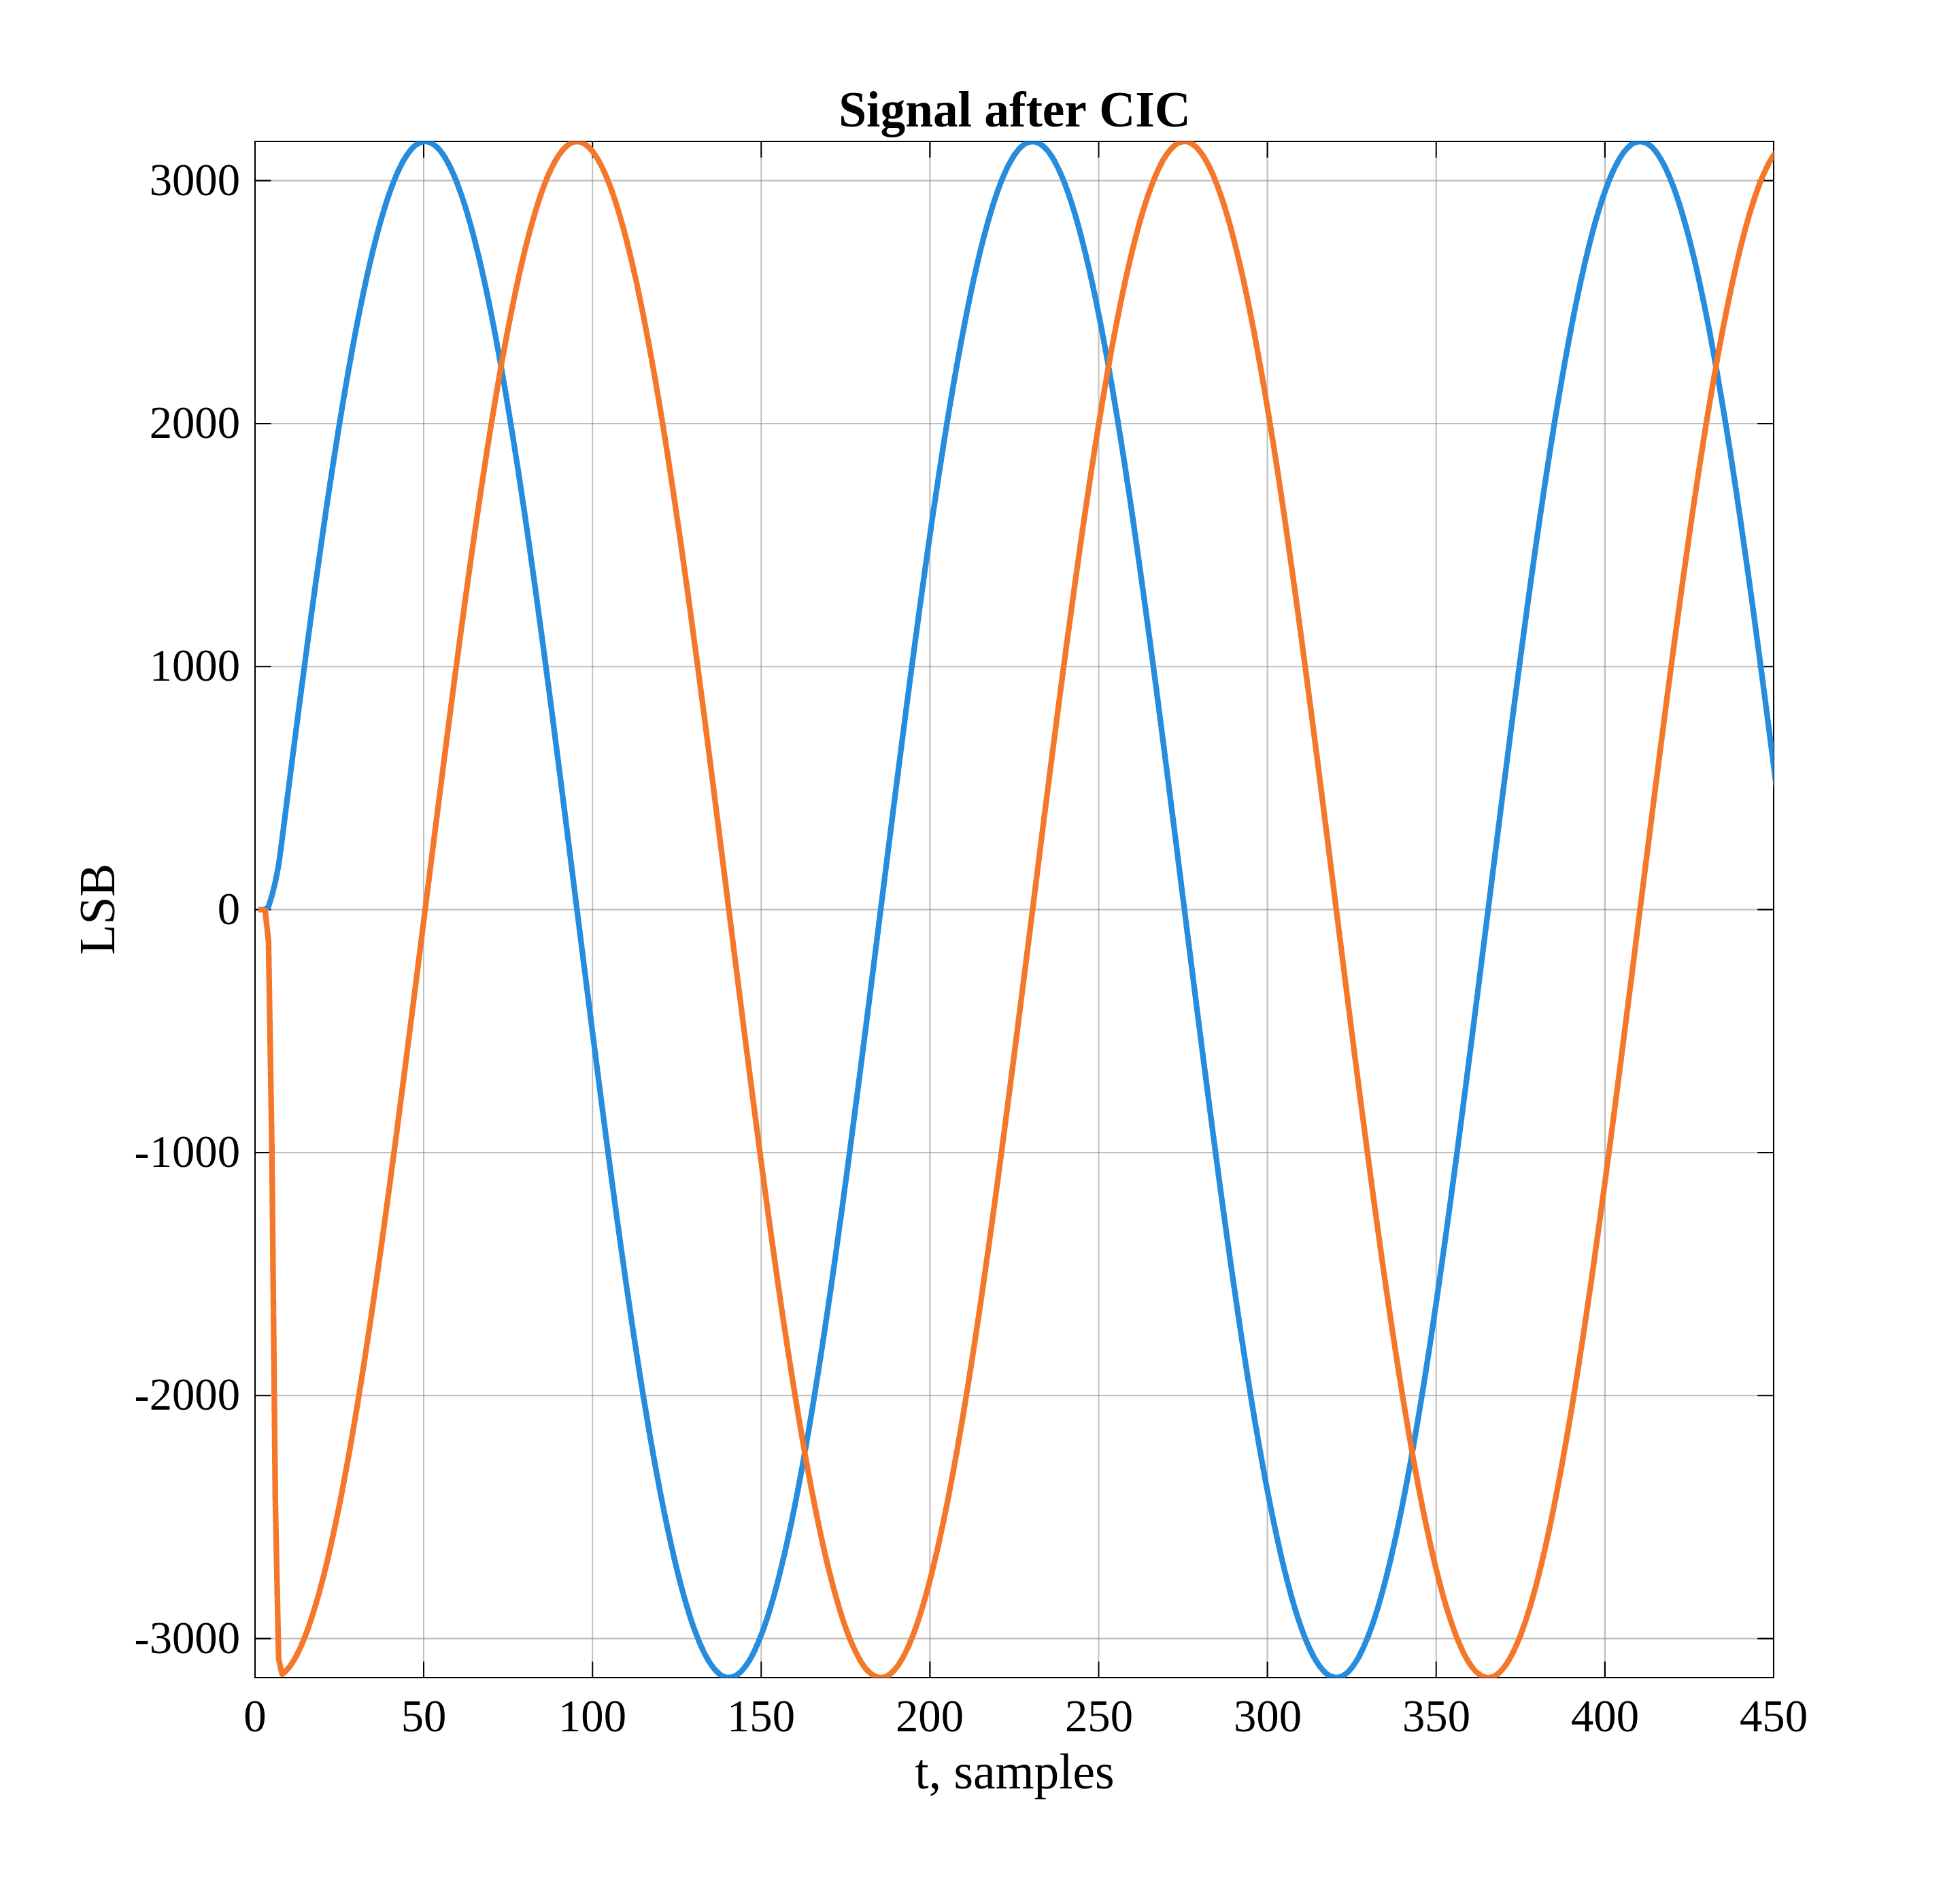
\includegraphics[width=\textwidth]{export_figs/p2_fig_09.png}
        \caption*{а) Осциллограмма}
    \end{minipage}\hfill
    \begin{minipage}{0.48\textwidth}
        \centering
        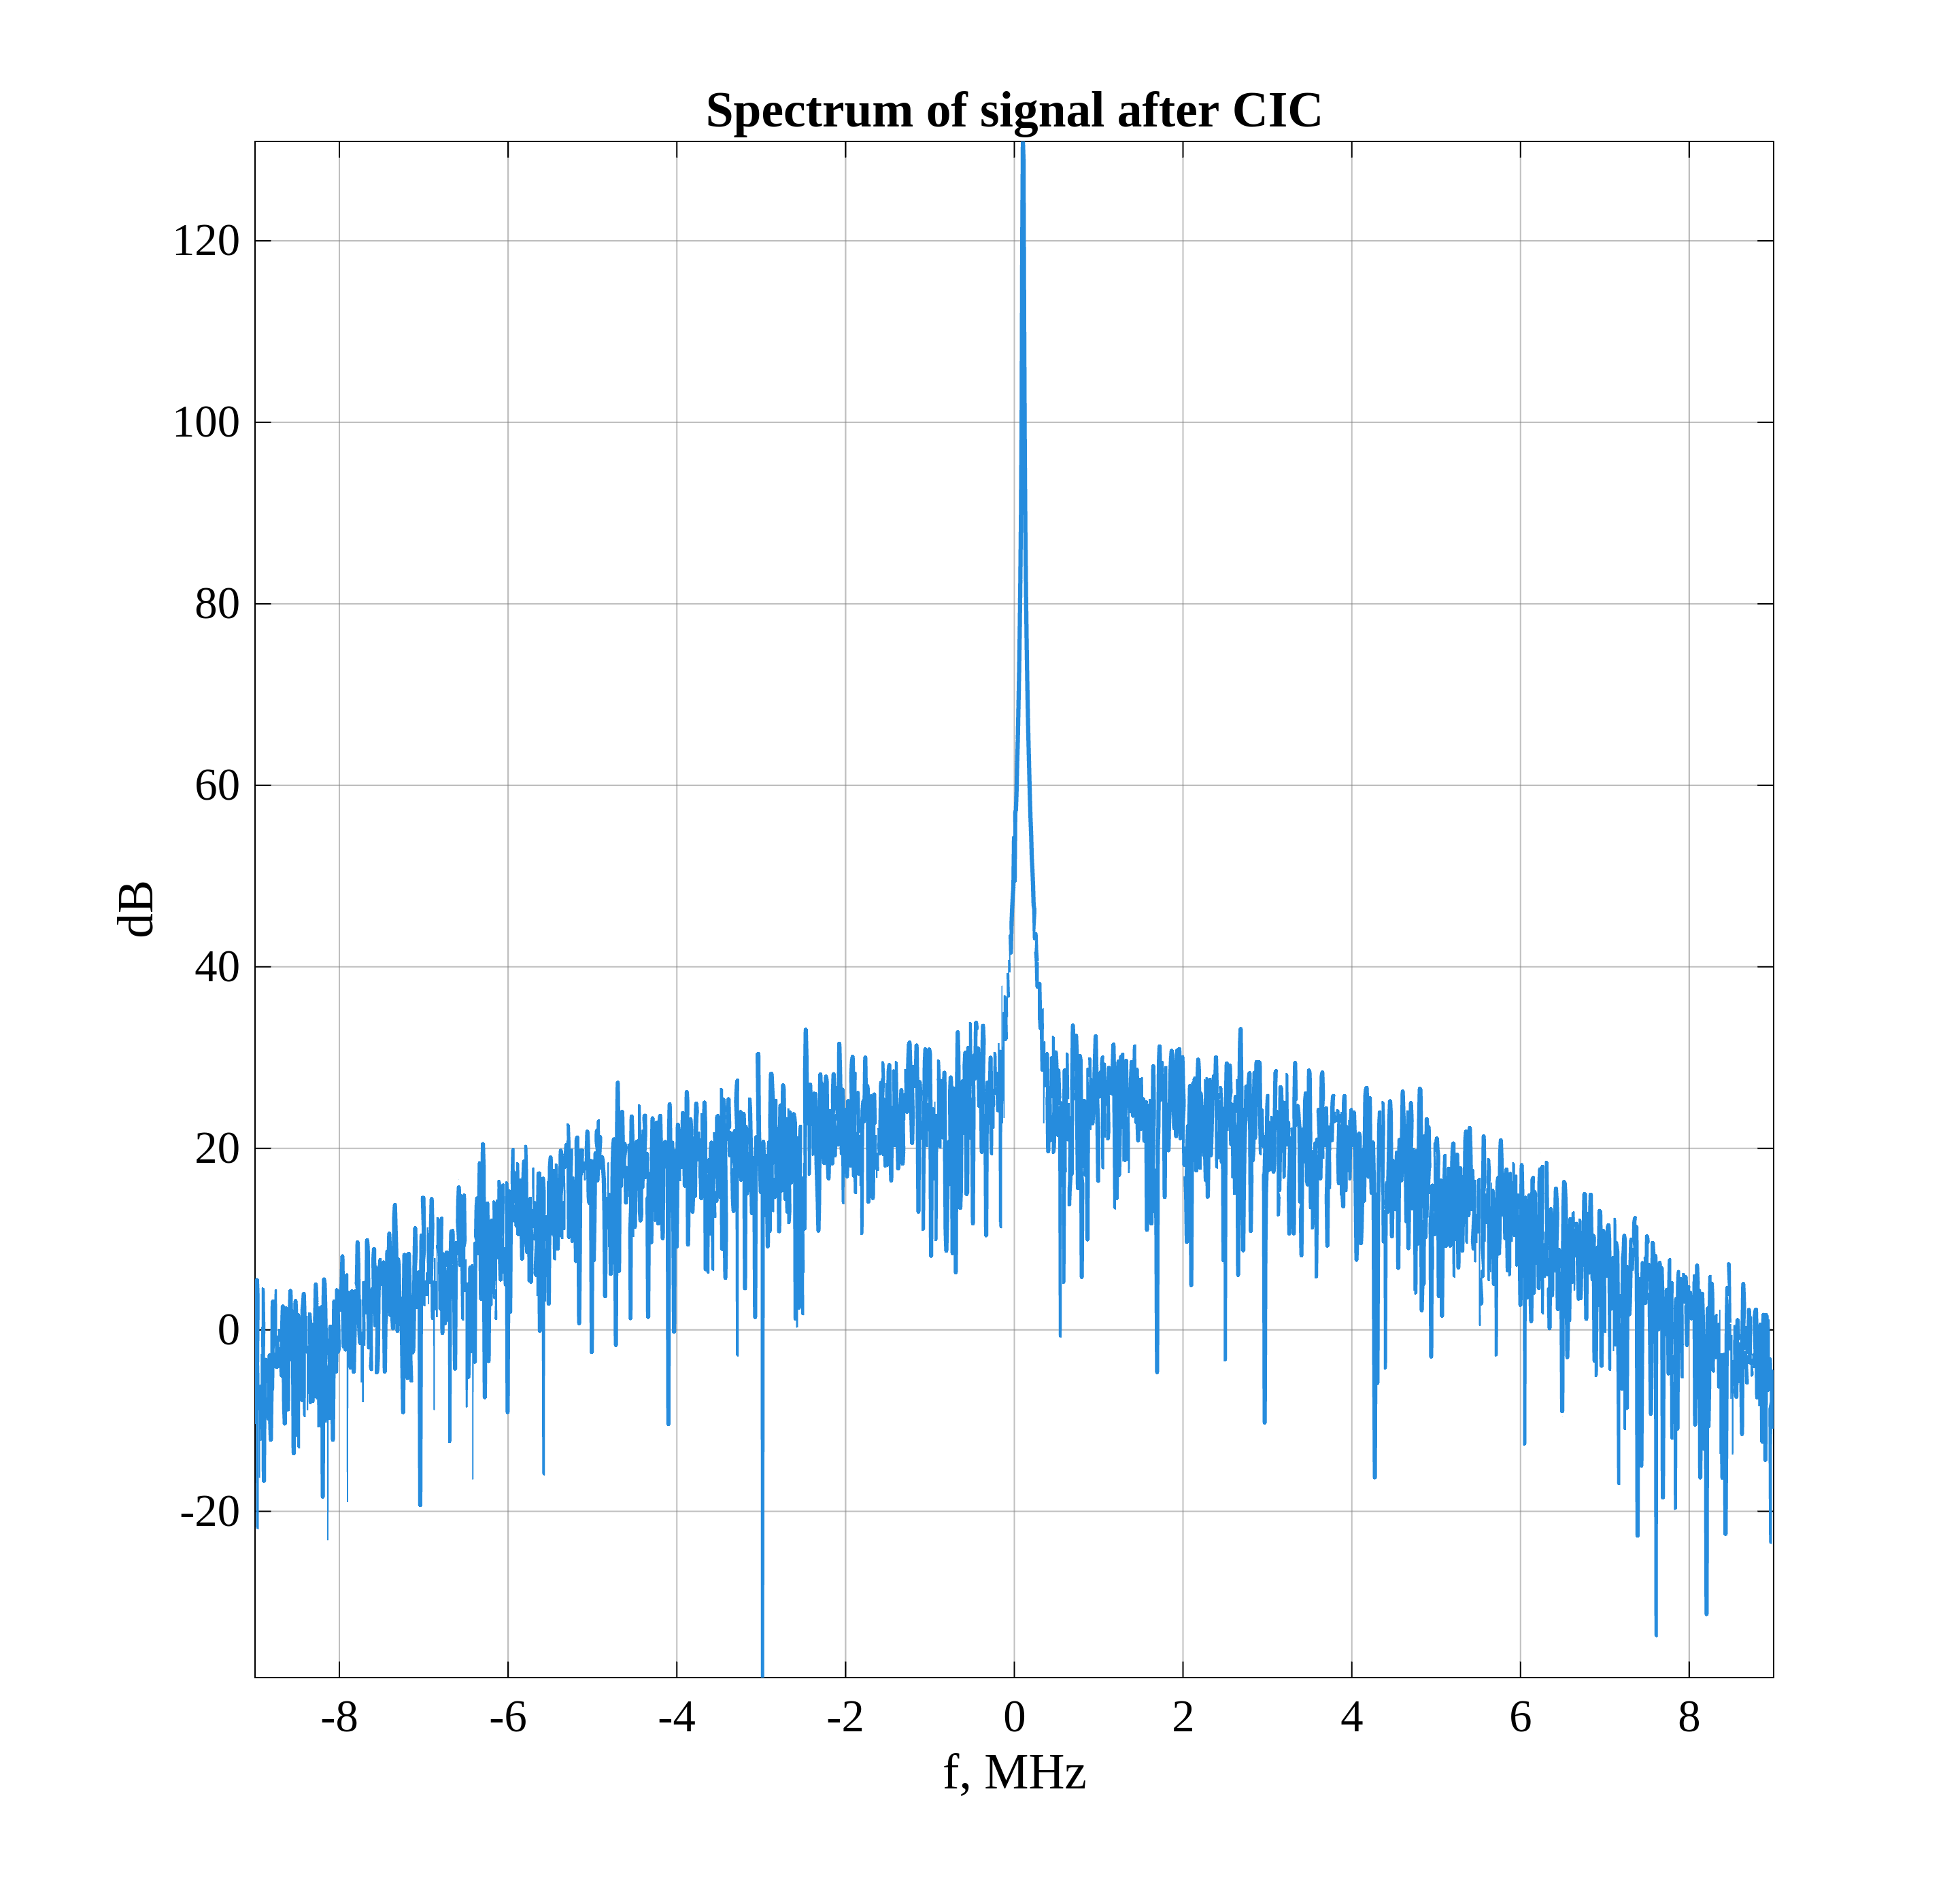
\includegraphics[width=\textwidth]{export_figs/p2_fig_10.png}
        \caption*{б) Спектр}
    \end{minipage}
    \caption{Сигнал после гребенчатого фильтра (CIC)}
    \label{fig:cic_out}
\end{figure}

Окончательное формирование частотной характеристики осуществляет корректирующий КИХ-фильтр (FIR). Он решает две задачи: выравнивает спад АЧХ первого каскада в полосе пропускания и обеспечивает крутой спад в переходной полосе с подавлением внеполосных компонент не менее 60 дБ. 

На рисунке \ref{fig:fir_out} представлены результаты фильтрации на выходе всего приемного тракта. На осциллограмме (рис. \ref{fig:fir_out}а), приведенной в сопоставимом масштабе со смещением относительно начального переходного процесса, наблюдается чистая синусоида без искажений. В спектре выходного сигнала (рис. \ref{fig:fir_out}б) отчетливо видна селективная полоса пропускания шириной около $7.5$ МГц: полезный сигнал на частоте $f_{IF} = +0.1$ МГц проходит без потерь, а спектральные составляющие в полосе заграждения (включая остатки на частоте $-6.1$ МГц) подавлены ниже уровня $-40$ дБ.

\begin{figure}[H]
    \centering
    \begin{minipage}{0.48\textwidth}
        \centering
        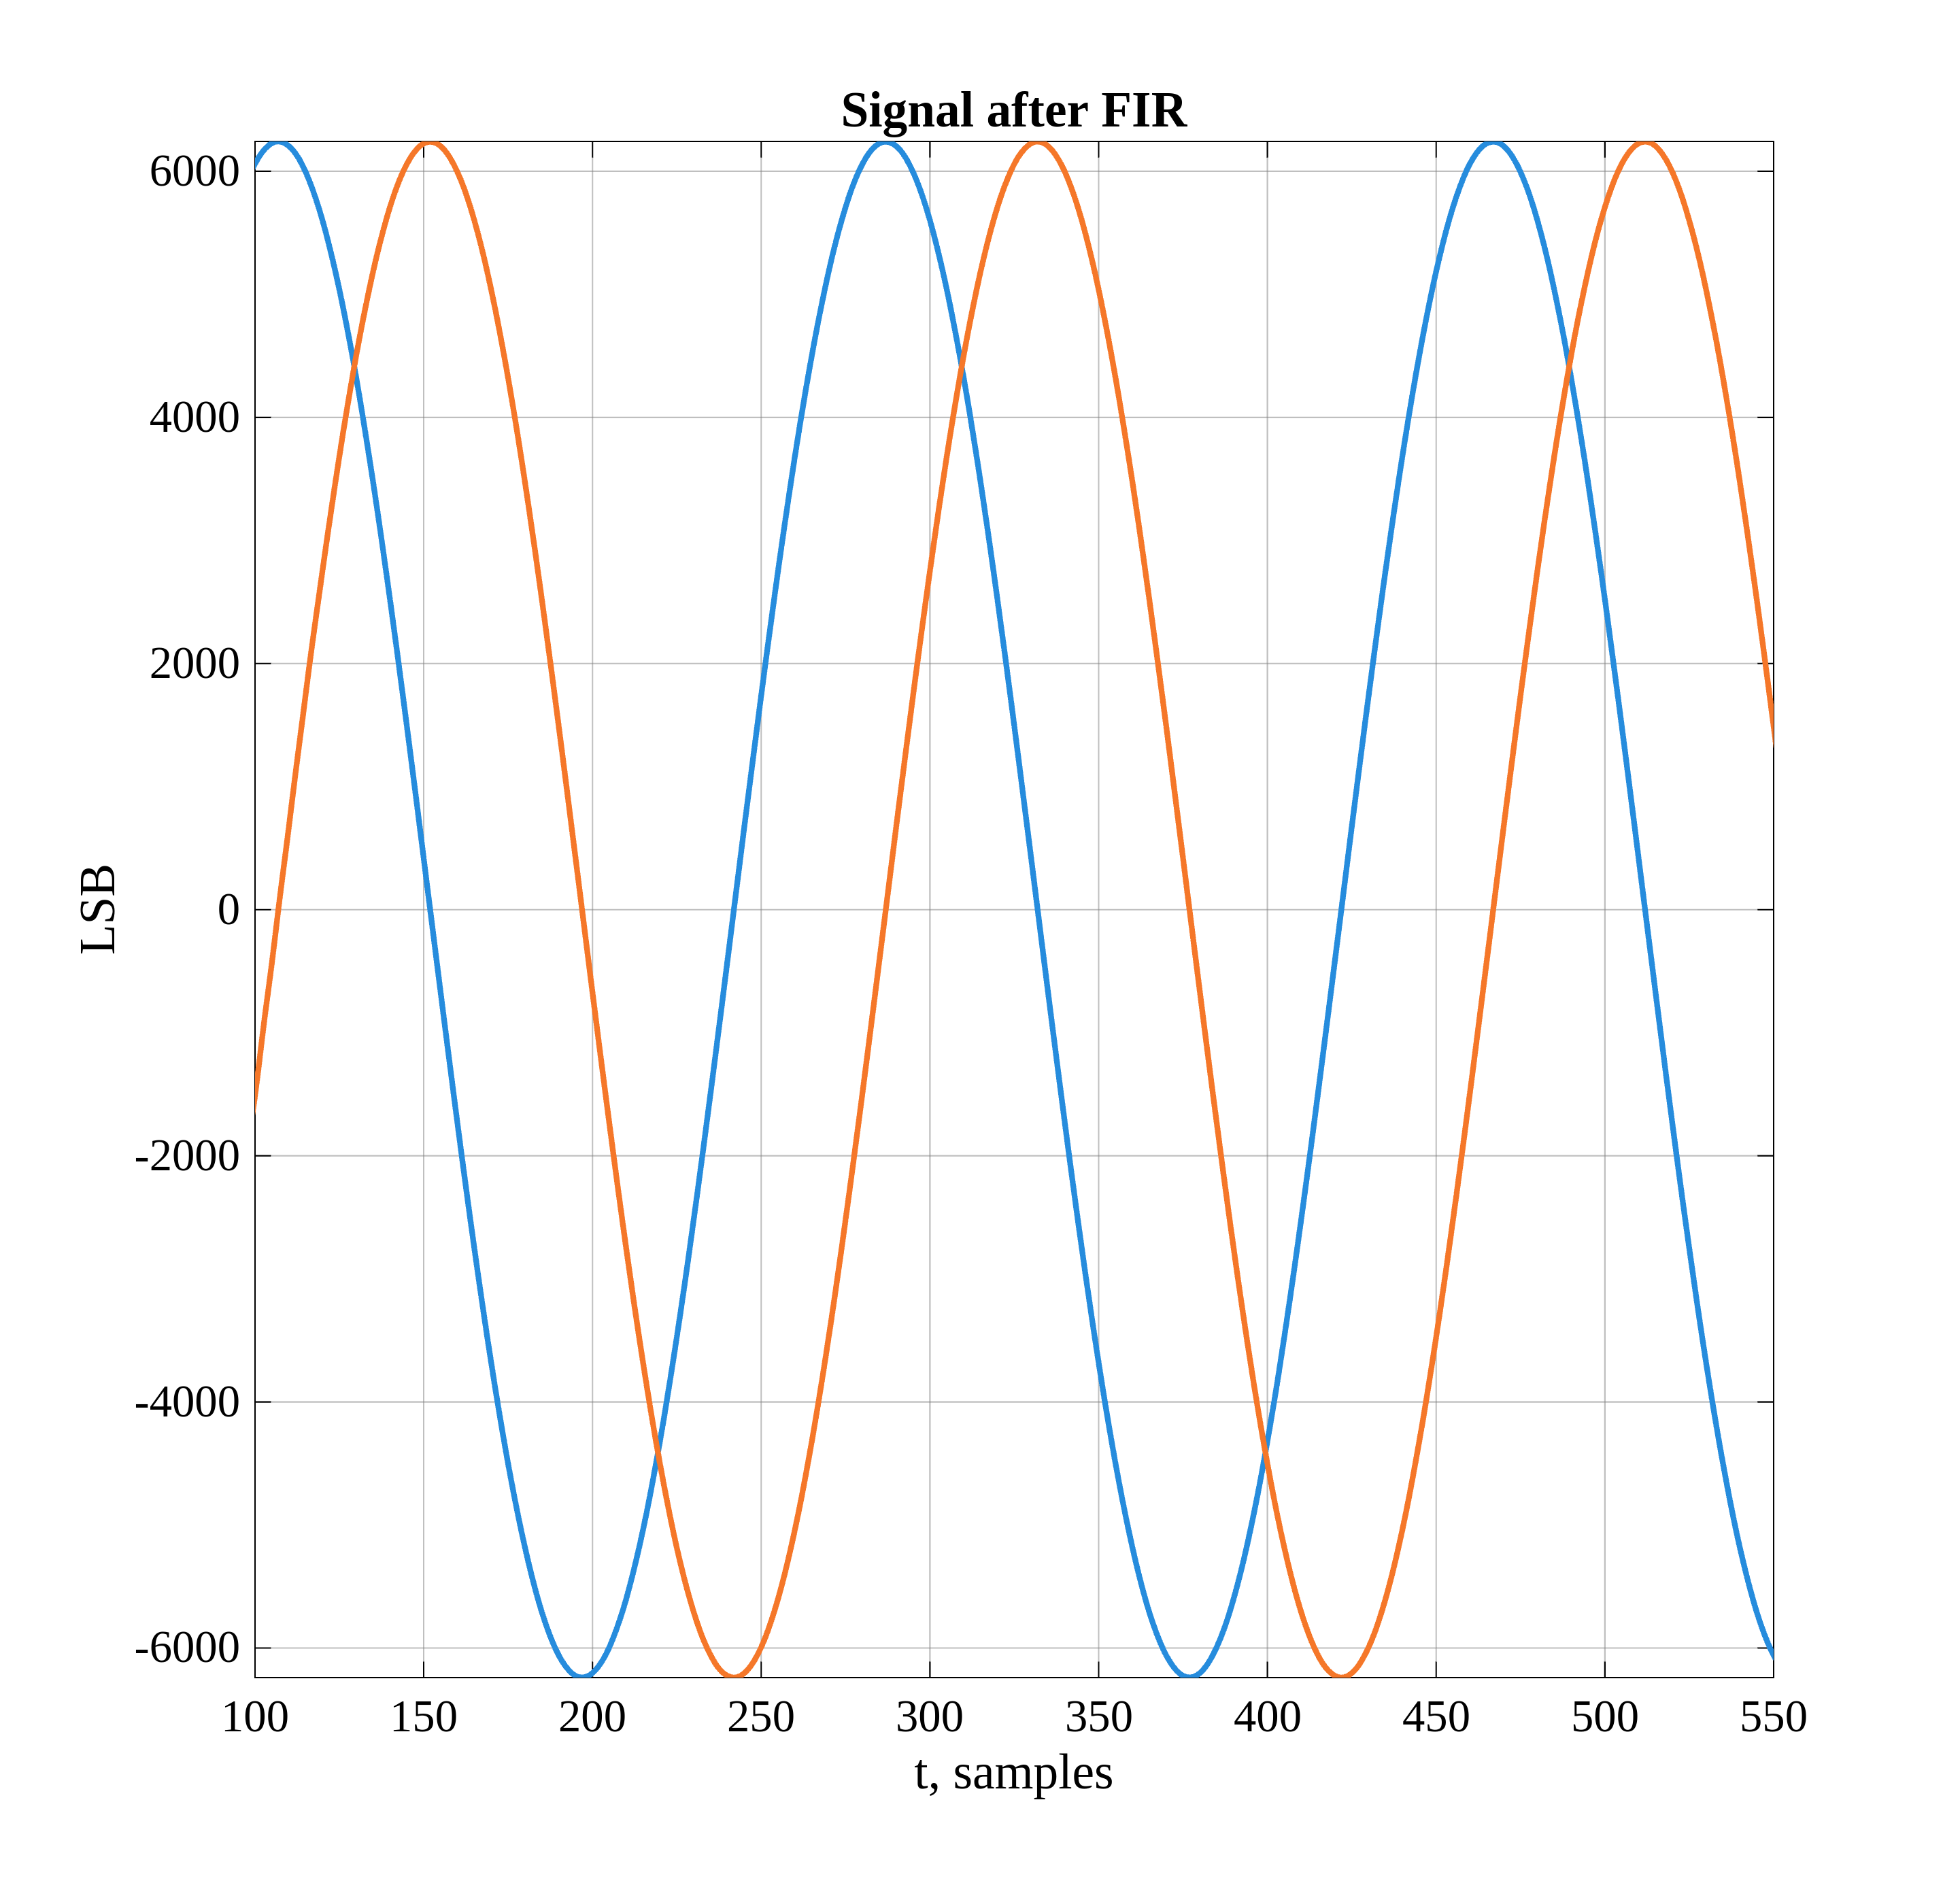
\includegraphics[width=\textwidth]{export_figs/p2_fig_11.png}
        \caption*{а) Осциллограмма}
    \end{minipage}\hfill
    \begin{minipage}{0.48\textwidth}
        \centering
        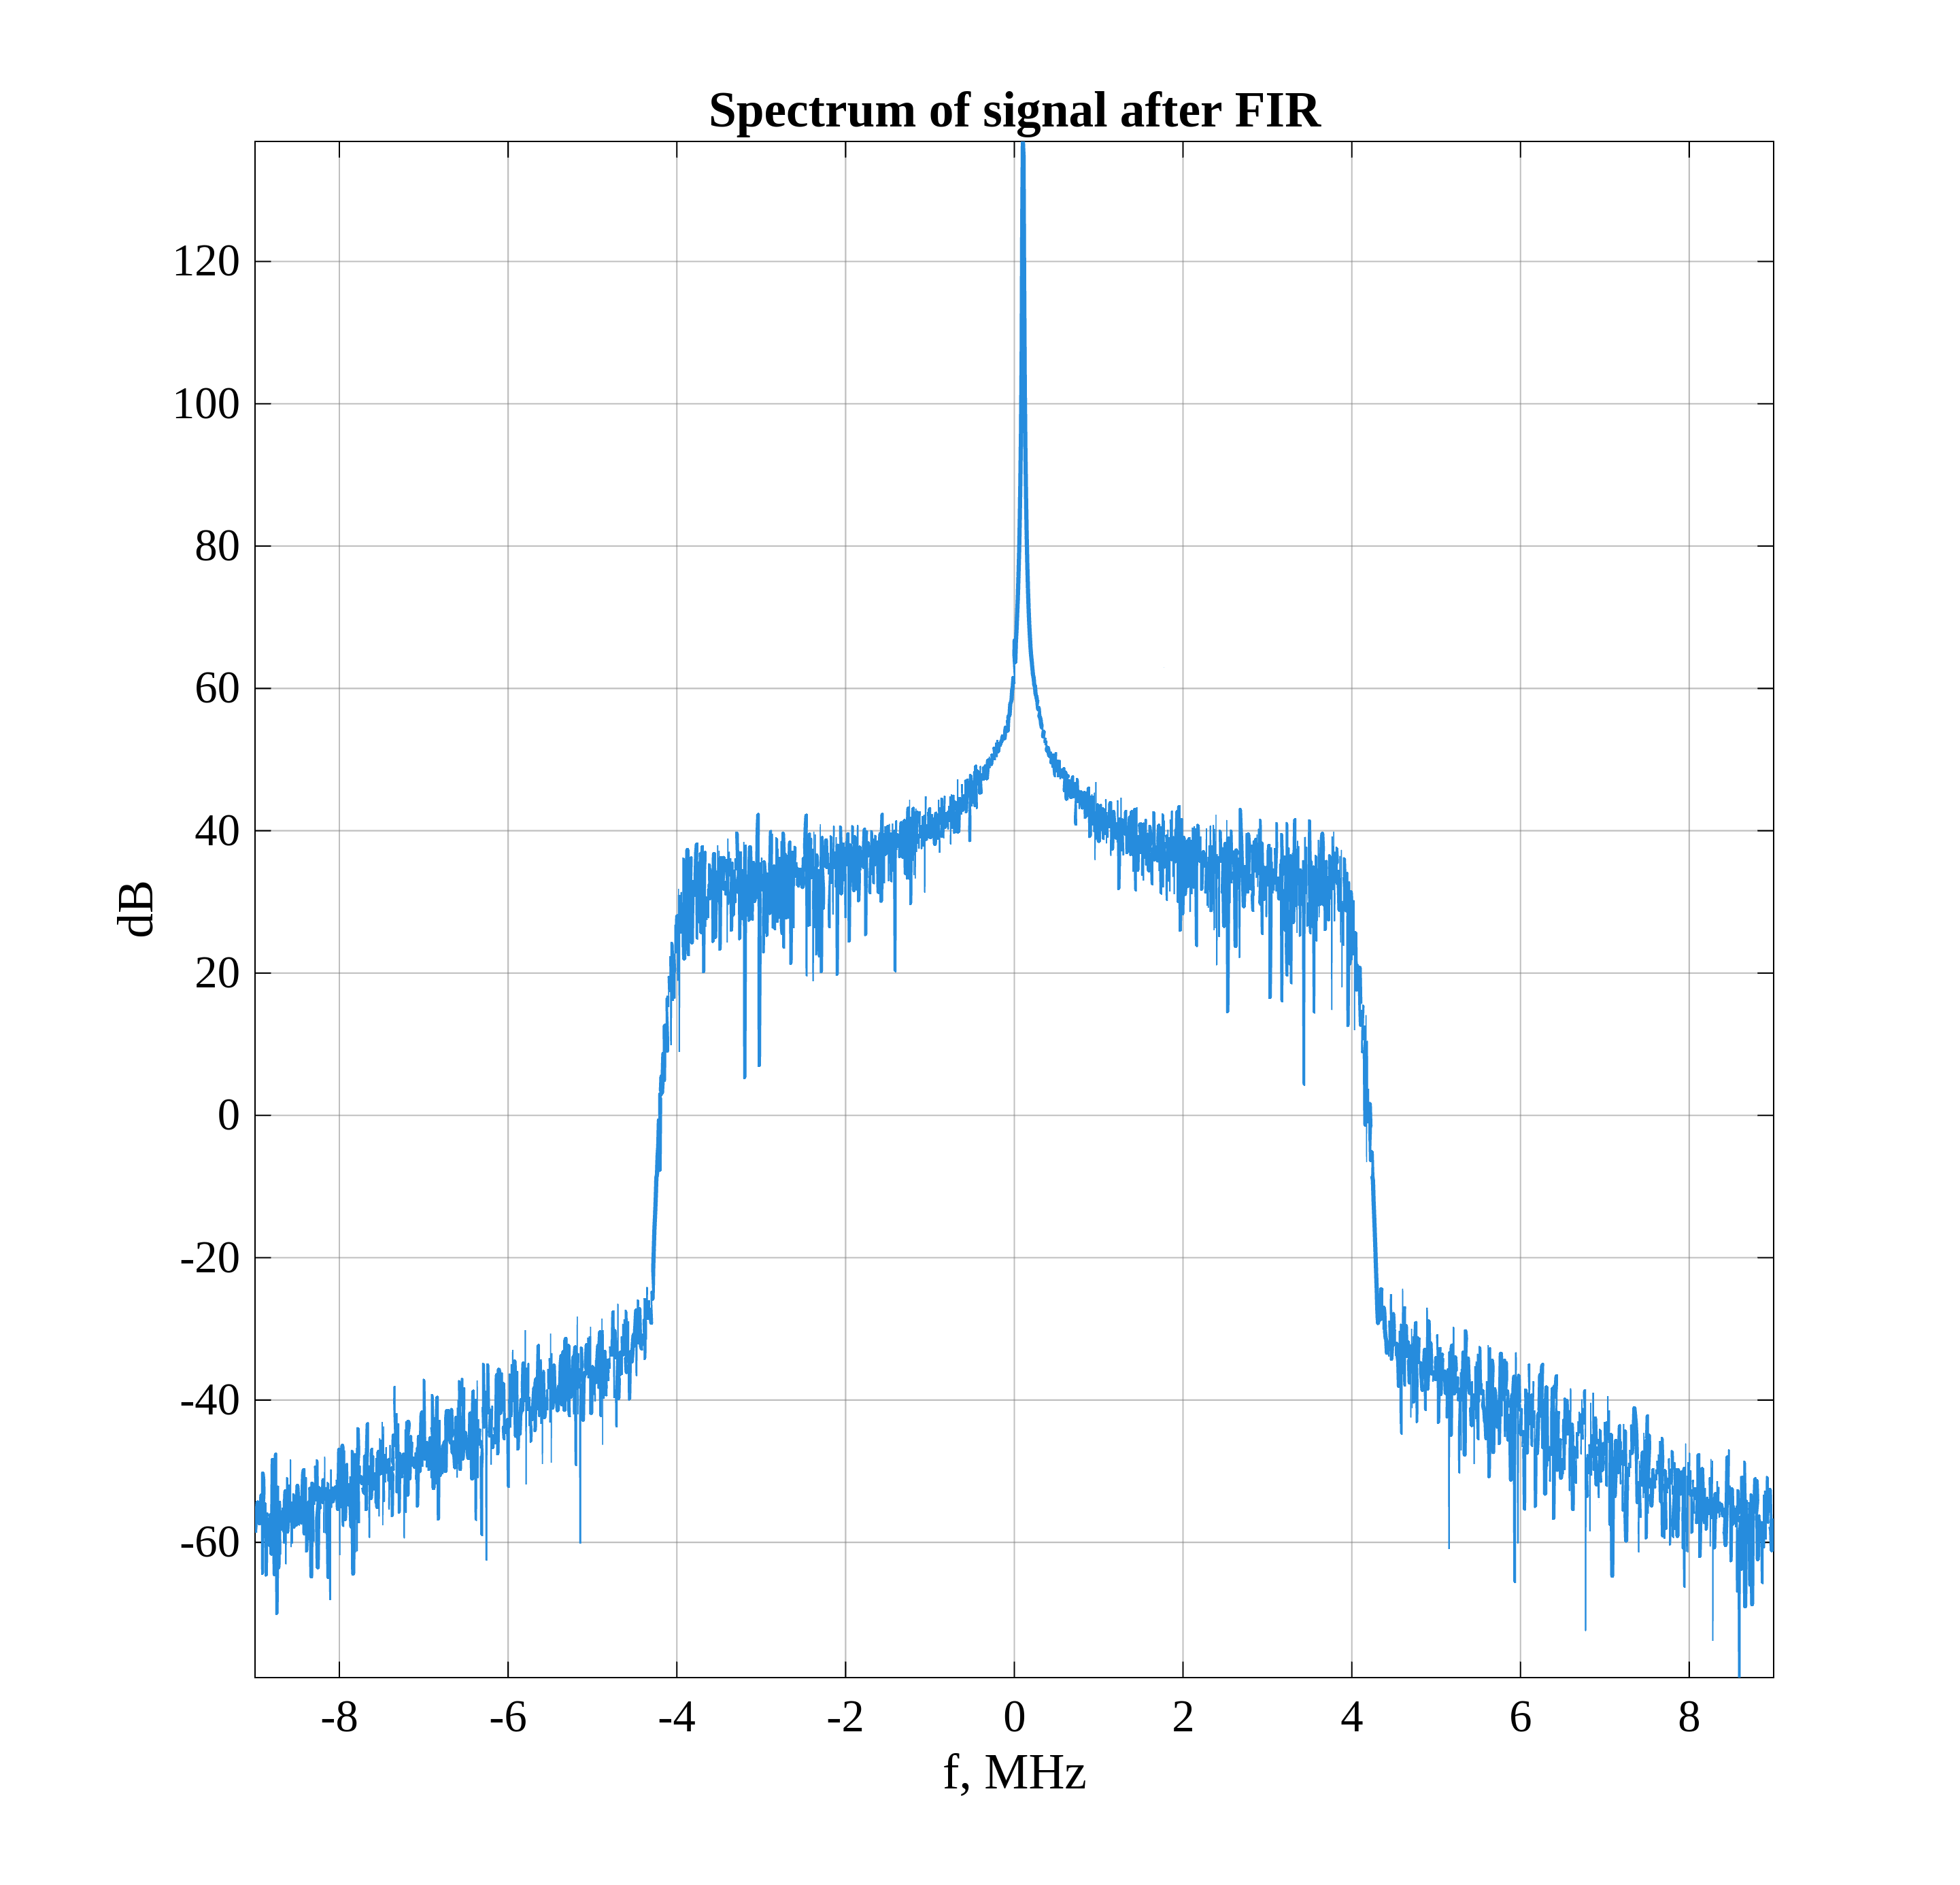
\includegraphics[width=\textwidth]{export_figs/p2_fig_12.png}
        \caption*{б) Спектр}
    \end{minipage}
    \caption{Сигнал на выходе устройства после компенсирующего КИХ-фильтра (FIR)}
    \label{fig:fir_out}
\end{figure}
